\documentclass{automatextcc}
\usepackage{ulem}
\usepackage{dsfont}
\usepackage{placeins}
\usepackage{refcheck}
\usepackage{enumitem}

\usepackage{xcolor}


% Caminho da Pasta das Figuras
\graphicspath{{figuras/}}

%\makeindex  Opcional (Índice Remissivo)

\newcommand{\nico}[1]{\textcolor{orange}{#1}}
\newcommand{\pumi}[1]{\textcolor{red}{#1}}
\newcommand{\R}{\mathds{R}}
\newcommand{\N}{\mathds{N}}


\newcommand{\bs}[1]{\boldsymbol{#1}}

\begin{document}


\title{Composição Automática de Músicas utilizando Redes Neurais Recorrentes}
\author{Nicolas Mathias Hahn}

% orientador(a) do trabalho {nome}{Orientador(a)}
\advisor{Prof. Dr. Guilherme Pumi}{Orientador}
% universidade onde obteve o título e atual
\advisorinfo{Doutor pela Universidade Federal do Rio Grande do Sul, Porto Alegre, RS}{UFRGS}

% banca examinadora:
\examinera{Prof. Dr. João Henrique Ferreira Flores}
\examinerainfo{Doutor pela Universidade Federal do Rio Grande do Sul, Porto Alegre, RS}{UFRGS}

% departamento:
\dept{\DEST}

% data de entrega:
\date{Outubro de 2022}


% Capa
\maketitulo

% Folha de rosto
\makefolhaderosto

% Folha de aprovação
\makefolhadeaprovacaoA % Um membro na banca
%\makefolhadeaprovacaoB % Dois membros na banca


% Epígrafe (OPCIONAL)
\newpage
\vspace*{\fill}
\begin{flushright} % mexer aqui
	\textit{``Since I have always preferred making plans to executing them, I have gravitated towards situations and systems that, once set into operation, could create music with little or no intervention on my part. That is to say, I tend towards the roles of planner and programmer, and then become an audience to the results.''} \newline
	\textit{Brian Eno \citep{alpern1995}}.
\end{flushright}

% Agradecimentos
\newpage
\chapter*{Agradecimentos}
Agradeço a xxx. Opcional % mexer aqui

% palavras chave
    % português
\keyword{Redes Neurais}
\keyword{Música}
    % inglês
\keyworde{Neural Networks}
\keyworde{Music}

% resumo 
    % português
\begin{abstract}
Este trabalho ....
\end{abstract}
    % inglês
\begin{englishabstract}
In this work ....
\end{englishabstract}

% sumário (Obrigatório)
\tableofcontents

% lista de ilustrações (Obrigatório)
\listoffigures

% lista de tabelas (Obrigatório)
\listoftables


%%%%%%%%%%%%%%%%%%%%%%%%%%%%%%%%%%%
%%%%  Introdução
%%%%%%%%%%%%%%%%%%%%%%%%%%%%%%%%%%%
\chapter{Introdução}


    % considerações iniciais | contexto histórico
Composição algorítmica, ou composição automática, refere-se ao processo de criação de músicas por meio de algum processo formal com pouca ou nenhuma intervenção humana. De acordo com \citet{maurer}, podemos encontrar três metodologias diferentes que existem em composição algorítmica: estocástica, \textit{rule-based} e inteligência artificial.

Wolfgang Amadeus Mozart (1756-1791) utilizou técnicas de composição algorítmica em sua obra \textit{Musikalisches Wurfelspiel} (\textit{Dice Music}), um jogo musical que envolvia atribuir um número para fragmentos de músicas, e combiná-los ao acaso, criando uma nova peça com as partes selecionadas. Além disso, John Cage (1912-1992), assim como Mozart, utilizou aleatoriedade em suas composições. Como exemplo, temos \textit{Reunion}, uma performance em que músicas são geradas ao jogar xadrez em um tabuleiro equipado com um foto receptor: cada lance emitia um som e, portanto, a música resultante é única por jogo. Por fim, com o auxílio de computadores, David Cope (1941-) criou, em 1981, o EMI (\textit{Experiments in Musical Intelligence}), um sistema baseado em grandes bases de dados com descrições de estilos de diferentes estratégias composicionais e, como complemento, o sistema também tinha a capacidade de criar as próprias regras composicionais por meio dos novos dados recebidos \citep{alpern1995, maurer}. 


    % tentar 2 parágrafos (jogando ideias por enquanto)
%Composição algorítmica, ou composição automática, refere-se ao processo de criação de músicas por meio de algum processo formal com pouca ou nenhuma intervenção humana. De acordo com \citet{maurer}, podemos encontrar três metodologias diferentes que existem em composição algorítmica: estocástica, \textit{rule-based} e inteligência artificial.

%Mozart, também, utilizou técnicas de composição automática em sua \textit{Musikalisches Wurfelspiel} (\textit{Dice Music}), um jogo musical que envolvia atribuir um número para cada pequeno fragmento de música, e combiná-los ao acaso, criando uma nova peça de parte selecionadas aleatoriamente. Essa simples forma de ``composição algorítmica'' deixa o processo criativo nas mãos do acaso, deixando o rolar de um dado decidir quais notas serão utilizadas \citep{alpern1995}.

%Existem exemplos modernos, também, de composição algorítmica sem o uso de computadores. Jogn Cage, por exemplo, assim como Mozart, utilizou aleatoriedade em muitas de suas composições, como em \textit{Reunion}, performada por jogar xadrez em um tabuleiro equipado com um foto receptor: Os lances dos ``jogadores'' disparavam sons, e portanto a peça musical é diferente a cada vez que um jogo é jogado \citep{alpern1995}. 

% http://artsites.ucsc.edu/faculty/cope/experiments.htm
%Um exemplo disso é o sitema de David Cope chamado de \textit{Experiments in Musical Intelligence - EMI}. EMI é baseado em uma grande base de dados de descrições de estilos, ou regras, de diferentes estratégias composicionais. No entanto, EMI também tem a capacidade de criar sua própria gramática e base de dados de regras, em que o próprio computador deduz baseado em diversas partituras de um compositor em específico que é inputado no sistema. EMI tem sido utilizado para composição musical automática com um certo sucesso em estilos similares ao de Bach, Mozart, Bartók, Brahms, Joplin e muitos outros compositores.

%-------------------------------------------------------------

%Mozart, too, used automated composition techniques in his Musikalisches Wurfelspiel ("Dice Music"), a musical game which "involved assembling a number of small musical fragments, and combining them by chance, piecing together a new piece from randomly chosen parts" (Alpern, 1995). This very simple form of "algorithmic" composition leaves creative decisions in the hands of chance, letting the role of a dice to decide what notes are to be used.

%There are more modern examples, as well, of algorithmic composition without the use of the computer. John Cage, for example, like Mozart, utilized randomness in many of his compositions, such as in Reunion, performed by playing chess on a photo-receptor equipped chessboard: "The players' moves trigger sounds, and thus the piece is different each time it is perfomed" (Alpern, 1995).

%An example of this is David Cope's system called Experiments in Musical Intelligence (EMI). Like the previous example of Shottstaedt and of Ebcioglu's CHORAL, EMI is based on a large database of style descriptions, or rules, of different compositional strategies. However, EMI also has the capactiy to create its own grammar and database of rules, which the computer itself deduces based on several scores from a specific composer's work that are input to it. EMI has been used to automatically compose music that evokes already somewhat successfully the styles of Bach, Mozart, Bartók, Brahms, Joplin, and many others.


    % literatura
Na literatura, encontramos diversos exemplos de trabalhos envolvendo composição musical automática. Os dados utilizados para o objetivo de composição podem vir tanto em formato de áudio \citep[como o de][]{kuang2021} quanto em formato de texto \citep[como o de][]{agarwala2017}. Ao mesmo tempo em que o trabalho de \citet{colombo2016} é claro em sua relação com a composição algorítmica, \citet{souza2018} é evasivo. Também, observou-se um foco em criação de músicas e avaliação das composições musicais, seja pela estrutura musical seja pela opinião de ouvintes referente à geração (se era musicalmente plausível). Por fim, os trabalhos de \citet{fernandez2013}, \citet{ji2020} e de \citet{olivan2021} são um sucinto resumo de abordagens e técnicas de inteligência artificial (como redes neurais artificiais) utilizadas para composição automática de músicas, assim como as formas de avaliação. 

% ideias presentes, falta organizar...
%Na literatura, os artigos de \citet{fernandez2013} e \citet{olivan2021} contêm, sucintamente, exemplos e explicações de diversas abordagens utilizando técnicas de inteligência artificial (como redes neurais) para composição musical. Apesar de estarem associados, nem todos os trabalhos envolvendo composição musical fazem a relação com a área de composição algorítmica (exemplos temos \citet{agarwala2017} e \citet{souza2018}).
%Dados utilizados para criação dos modelos são tanto em formato de áudio quanto em formato de texto.
%Similar a linguagem, música atua como uma forma de expressão na qual combinações de notas musicais são capazes de comunicar um escopo de emoções (presente em \citet{agarwala2017}).
%Como em linguagem escrita, o processo de composição musical é um processo complexo que depende de um grande número de decisões (presente em \citet{olivan2021}).
%Em geral, os artigos não focam na avaliação do modelo, e sim no fato de que uma música é gerada de forma automática.


    % problematização | objetivos | hipóteses | justificativa
%\section{\sout{Problematização | Objetivos | Hipóteses } }
%\begin{itemize}
%    \item modelos que criam músicas mas com dificuldade de serem comparados
%    \item não apenas compor músicas de forma automática, mas também ser capaz de avaliar esses modelos de forma métrica (entropia e perplexidade) 
%\end{itemize}

O presente trabalho propõe-se a explorar o problema de composição algorítmica no contexto de modelagem, sendo as peças musicais geradas uma consequência dos modelos. Dessa forma, mesmo sem conhecimentos sobre teoria musical, é possível elencar um melhor modelo apenas por métricas objetivas. Por meio de técnicas de Processamento de Linguagem Natural e de Redes Neurais Artificiais, serão criados modelos capazes de composição com base em conjuntos de músicas na notação ABC. Consequentemente, os dados utilizados serão restritos ao formato textual. 
% O QUE MAIS INSERIR?
% COMO INSERIR?

%
% - talvez inserir mais detalhes sobre quais técnicas utilizadas
% - detalhar um pouco mais sobre o que foi (redes recorrentes, modelos de linguagem)
% - não foi falado quais artigos eu me baseio (abrir mais o parágrafo)
% - explicar talvez o impacto da modificação dos hyperparâmetros


%Mesmo \citet{olivan2021} sendo claros nas formas de avaliação de modelos de redes neurais que geram músicas, bem como nas formas de avaliação das músicas geradas, os trabalhos, no geral, concentram-se na criação das músicas e não na avaliação dos modelos. Posto isso, o presente trabalho propõe-se a explorar o problema no contexto de modelagem, sendo a composição algorítmica uma consequência do modelo. Dessa forma, mesmo sem conhecimentos sobre teoria musical, é possível elencar um melhor modelo apenas por métricas objetivas. No caso, entropia cruzada e perplexidade. Por fim, no contexto deste trabalho, estaremos nos restringido a dados no formato textual. 
% verificar melhor os artigos referente a algumas afirmações feitas nesse trecho...
%\pumi{Sugestão: introduzir melhor e então: ... a literatura,  no geral, concentram-se na criação das músicas e não na avaliação dos modelos... blabla uma excessão é o trabalho de \citet{olivan2021} blabla }

%\pumi{No geral falta trabalhar mais na intro. Precisa trabalhar mais na problematização e na descrição velada dos objetivo do trabalho, enfatizando os pontos importantes; }
% referencial teórico
\chapter{Referencial Teórico}


\section{Composição Algorítmica}
Composição algorítmica, ou composição automática, refere-se ao processo de criação de músicas por meio de algum processo formal com pouca ou nenhuma intervenção humana. O termo ``algoritmo'' é definido como um conjunto predeterminado de instruções com o objetivo de resolver um problema em específico com um número limitado de passos. O ``problema'' encarado por compositores é a composição musical, e as ``instruções'' predeterminadas sugerem que, uma vez que o processo é iniciado, a intervenção humana é substituída. Portanto, ``composição automática'' também descreve adequadamente esse tipo de composição musical, sendo que ``automático'' refere-se a ``qualquer coisa que pode se mover ou agir por conta própria'' \citep{alpern1995, maurer}.

De acordo com \citet{maurer}, podemos encontrar três metodologias diferentes que existem em composição algorítmica: 
\begin{itemize}
    \item \textbf{estocástica:} abordagem mais simples. Envolve aleatoriedade e pode ser tão simples quanto gerar uma série de notas musicais ao acaso, bem como sortear uma ordem de fragmentos de músicas para ser performada pelo músico.
    \item \textbf{\textit{rule-based}:} em vez de delegar decisões ao acaso como no método estocástico, um sistema \textit{rule-based} define uma ``constituição'' ou ``gramática'' (sistema formal de princípios ou regras que as possíveis frases de uma linguagem são geradas) em que o sistema deve seguir uma vez iniciado o processo de composição. 
    \item \textbf{inteligência artificial (IA): }similar ao ``rule-based'' no sentido de ser baseado em uma gramática pré-definida. No entanto, sistemas de IA têm a capacidade de definirem sua própria gramática, que pode evoluir (isto é, ser modificada de uma forma automática) ao longo do processo.
\end{itemize}
Mais detalhes podem ser encontrados em \citet{alpern1995}, \citet{maurer}, \citet{nierhaus2009}, \citet{fernandez2013} e \citet{olivan2021}.  

% - no escopo deste trabalho, vamos focar no 3º tipo bla bla


    % NN
\section{Redes Neurais Artificiais}
    % aggarwal 2018
%Redes Neurais Artificiais são técnicas populares de aprendizagem de máquina que simulam o mecanismo de aprendizagem presente em organismos vivos.
    % haykin 2002
%O trabalho em redes neurais artificiais, usualmente denominadas "redes neurais", tem sido motivado desde o começo pelo reconhecimento de que o cérebro humano processa informações de uma forma diferente do computador digital convencional. O cérebro é um computador (sistema de processamento de informação) altamente complexo, não linear e paralelo. Ele tem a capacidade de organizar seus constituintes estruturais, conhecidos por neurônios, de forma a realizar certos processamentos (ex. reconhecimento de padrões, percepção e controle motor) muito mais rapidamente que o mais rápido computador digital hoje existente.
    % elements of statistical learning 2008
%O termo "rede neural" tem evoluído para abranger uma grande classe de modelos e métodos de aprendizagem. [...] Elas são apenas modelos estatísticos não lineares.
    % goodfellow 2016
%Alguns dos algoritmos iniciais que reconhecemos hoje tinham o intuito de ser um modelo computacional da aprendizagem biológica, i.e., modelos de como a aprendizagem poderia ocorrer no cérebro. A correspondente perspectiva de deep learning (redes neurais artificiais) é que são engineered systems inspirados pelo cérebro (seja humano seja de outro animal)
    % hair et al 2005
%Redes neurais são uma abordagem totalmente diferente para a análise de dados em relação a qualquer outra técnica multivariada. Em vez de conceitualizar o problema como de caráter matemático, redes neurais usam o cérebro humano e sua estrutura para desenvolver uma estratégia de processamento. Apesar de jamais sermos capazes de construir redes neurais tão complexas quanto o cérebro humano, podemos usar seus princípios básicos de unidades de processamento paralelo múltiplo engajadas no reconhecimento de padrões. 

% paragrafo
Redes Neurais Artificiais (RNA) são técnicas de aprendizagem de máquina inspiradas no mecanismo de aprendizagem presente em organismos vivos \citep{aggarwal2018} sendo que, nos seus primórdios, os algoritmos tinham o intuito de ser um modelo computacional capaz de imitar a aprendizagem ocorrida no cérebro \citep{goodfellow2016}.  Por outro lado, tecnicamente RNAs podem ser vistas como modelos estatísticos não lineares \citep{hastie2009}.


\subsection{\nico{Redes Neurais e a Estatística}}
Muitos modelos de RNAs são similares ou idênticos a populares técnicas estatísticas como modelos lineares generalizados, regressão linear (simples e múltipla), regressão polinomial, regressão não paramétrica e análise discriminante (como a regressão logística), especialmente quando a ênfase é na predição de um fenômeno complexo em vez de sua explicação. \nico{Devido a esse foco em predição, RNAs são utilizadas como modelos \textbf{caixa preta}: uma certa entrada produz uma determinada saída da função, mas o processo interno que a rede utilizou para chegar nesse resultado é desconhecido e, consequentemente, há perda de interpretabilidade do modelo \citep{sarle1994, cheng1994, rojas1996}}.

No contexto de RNAs, é possível definir dois procedimentos para a resolução de algum problema prático (aplicado): \nico{especificar a arquitetura da rede e treinar a rede com um conjuntos dados de treinamento. Paralelamente, no contexto estatístico, esses passos são equivalentes a especificar um modelo e estimar seus parâmetros dado um conjunto de dados. Posto isso, apresentamos uma lista de termos comumente utilizados na literatura de RNAs e as respectivas equivalências de acordo com a estatística:}
\begin{itemize}
    \item variáveis são chamadas de atributos \nico{(\textit{features})};
    \item variáveis independentes são chamadas de entrada (\textit{input});
    \item valores preditos são chamados de saída (\textit{output});
    \item variáveis dependentes são chamadas de variáveis alvo (\textit{target}) ou valores de treinamento;
    \item resíduos são chamados de erros;
    \item estimação é chamada de treinamento, aprendizagem, adaptação ou auto-organização (\textit{self-organization});
    \item um critério de estimação é chamado de função erro ou de função custo;
    \item observações são chamadas de padrões (\textit{patterns}) ou de pares de treinamento (\textit{training pairs});
    \item parâmetros estimados são chamados de pesos (sinápticos);
    %\item interações são chamadas de neurônios de alta ordem (\textit{higher-order neurons});
    \item transformações são chamadas de links funcionais (\textit{functional links});
    %\item regressão e análise discriminante são chamados de aprendizagem supervisionada ou heteroassociação; \pumi{Aprendizagem supervisionada é um conceito mais geral que isso}
    %\item redução de dimensionalidade (\textit{data reduction}) é chamada de aprendizagem não supervisionada, codificação (\textit{encoding}) ou autoassociação;
    %\item análise de agrupamento (\textit{cluster analysis}) é chamada de aprendizagem competitiva ou quantização adaptativa de vetor  (\textit{adaptative vector quantization}); \pumi{esta erminologia nunca tinha visto}
    \item interpolação e extrapolação são chamadas de generalização.
\end{itemize}
Os termos estatísticos \textbf{amostra} e \textbf{população} não demonstram conter equivalentes na literatura de RNAs. No entanto, os dados são comumente divididos em conjunto de treino e de teste para validação cruzada \citep{cheng1994}.


\subsection{Neurônio}
Um neurônio (ou nó computacional) é uma unidade de processamento de informação fundamental para a operação de uma rede neural \citep{haykin2009}. Podemos identificar três elementos básicos do modelo neuronal:
\begin{enumerate}
    \item Um conjunto de sinapses, cada uma caracterizada por um peso ou força própria. O peso sináptico de um neurônio artificial pode estar em um intervalo que inclui valores positivos e negativos.
    \item Um \textit{somador} ou \textit{acumulador} para somar os sinais de entrada, ponderados pelas respectivas sinapses de cada neurônio, constituindo uma \textit{combinação linear}.
    \item Uma \textit{função de ativação} para restringir a amplitude de saída de um neurônio (fixando em um valor finito).
\end{enumerate}
Também é incluído um intercepto no modelo, chamado de \textit{bias} na literatura de \textit{machine learning}, com o intuito de aumentar ou diminuir o sinal de entrada da função de ativação, dependendo do seu sinal.

Dada uma sequência $x_1,\cdots,x_m$ de dados de entrada (valores observados) e uma função de ativação $\varphi(\cdot)$, a descrição do $k$-ésimo neurônio em uma rede neural nada mais é do que a determinação da função que leva o vetor de entrada $(x_1,\cdots,x_m)$ na $k$-ésima saída $y_k$. Uma configuração simples de um neurônio é dada pelo sistema de equações:
\begin{align*}
    u_k & := \sum_{i=1}^{m} w_{k,i}x_i;\\   
    y_k & := \varphi(u_k + b_k),
\end{align*}
sendo $b_k$ o \textit{bias} e $w_{k,i} \in \R$ os pesos associados ao neurônio.

\begin{figure}
    \centering
    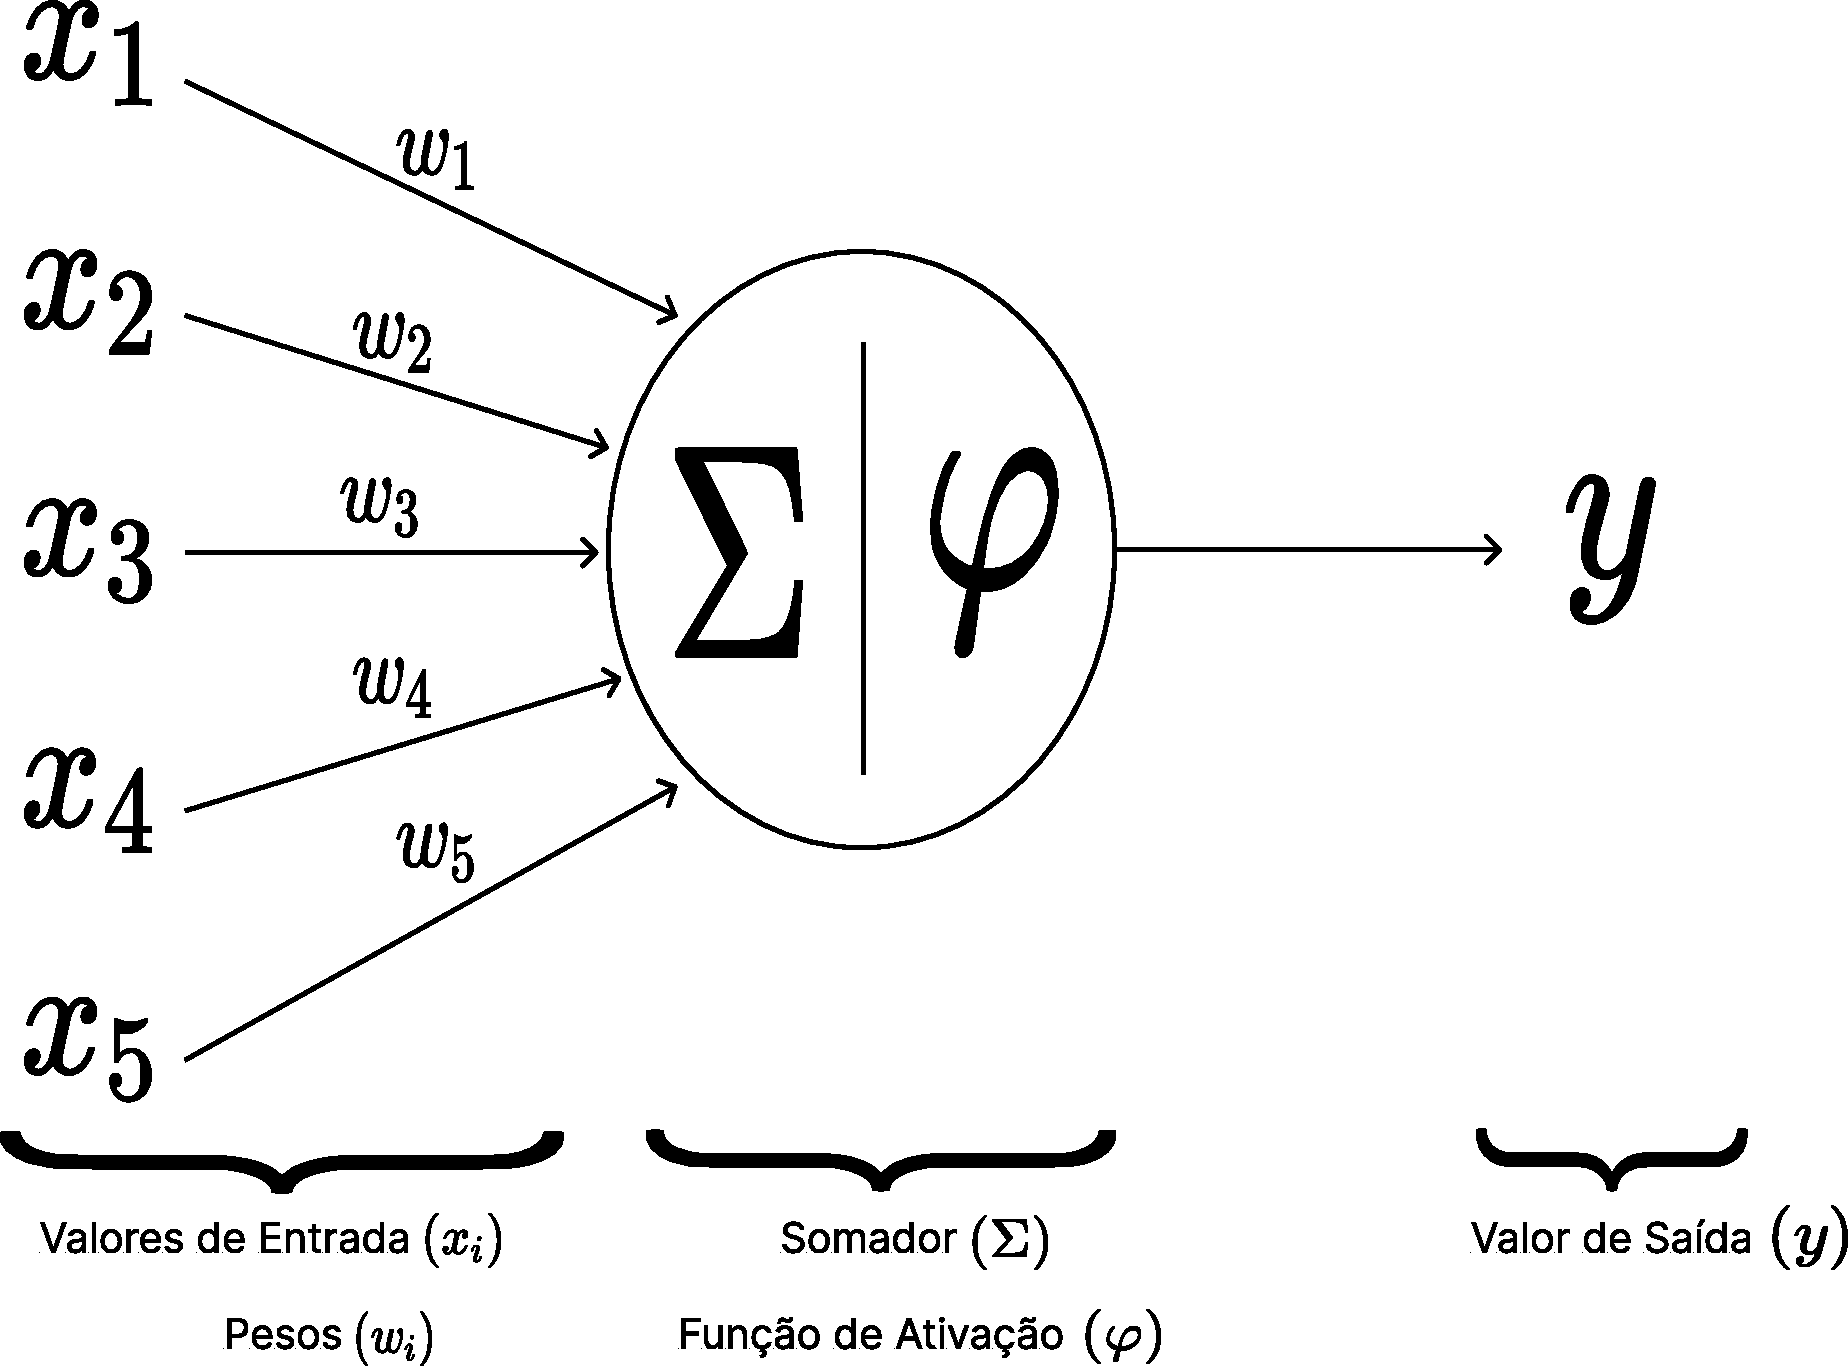
\includegraphics[width=.7\textwidth]{figuras/neuron_model.pdf}
	\caption{Modelo Neuronal \citep[adaptado de][]{haykin2001,hair2005}}
\end{figure}

\subsection{\nico{Função de Ativação}}
\nico{Uma função de ativação pode ser linear ou não linear. A escolha de uma particular função de ativação depende do problema que o neurônio almeja resolver. Abaixo, seguem algumas funções de ativação:}

%O objetivo da função de ativação é determinar se a informação que o neurônio está recebendo será passada adiante ou será ignorada \citep{dsa2022}. \citet{hagan2014} comenta que uma função de ativação particular é selecionada para satisfazer uma determinada especificação do problema que o neurônio almeja resolver. Assim, temos que a função de ativação pode ser linear ou não-linear. Abaixo, seguem algumas funções de ativação:

%\pumi{Minha sugestão: A função ativação é muito importante por que isto e aquilo blabla. Sua escolha portanto é muito importante blabla e uma função particular é escolhida por que blabla o suporte da função em geral determina blabla Algo nessas linhas. Existem vários tipos de função de ativação, como por exemplo:}
% referente ao parágrafo
% - funções são escolhidas para resolver problemas específicos
% - peculiaridades para cada perfil de rede

\begin{itemize}
    \item \textbf{linear:} $f: \R \rightarrow \R$ dada por 
    \[f(x) := \alpha x, \quad \alpha \in \R\backslash\{0\}.\]
    Observe que no caso da função linear, o neurônio está sempre ativado, sendo seu valor alterado pela constante $\alpha$. Em particular, quando $\alpha=1$, temos a função identidade e, consequentemente, um modelo de regressão linear.
    \item \textbf{sigmóide ou \textit{logit}}: $f: \R \rightarrow (0,1)$ dada por 
    \[f(x) := \frac{1}{1 + e^{-x}}.\]
    Quando essa função de ativação é associada a uma rede, o neurônio é equivalente a uma regressão logística. Dessa forma, notamos que a função de ativação tem um papel semelhante à função de ligação no contexto de modelos lineares generalizados: relacionar o preditor linear ao respectivo valor esperado \citep{sarle1994,frei2020,mccullagh1989}.
    \item \textbf{tangente hiperbólica (\textit{tanh}):}  $f:\R \rightarrow (-1,1)$ dada por 
    \[f(x) := \frac{e^{x}-e^{-x}}{e^{x}+e^{-x}}.\]
    Em contextos que uma função sigmoidal é necessária (como a predição de uma variável binária), a \textit{tanh} tipicamente performa melhor. Vale comentar que funções de ativação sigmoidal são mais comuns em estruturas diferentes que a de redes alimentadas adiante, como as redes recorrentes \citep{goodfellow2016}.  
    \item \textbf{ReLU (\textit{Rectified Linear Unit}):} $f: \R \rightarrow [0,\infty)$ dada por 
    \[f(x) := \max\{0,x\}.\]
    De acordo com \citet{goodfellow2016}, é a recomendação padrão para redes neurais modernas. O autor justifica que, por ser uma função quase linear, são preservadas muitas propriedades que fazem os modelos lineares bons generalizadores. 
    \item \textbf{\textit{softmax}}: $f:\R^n\rightarrow (0,1)^n$ dada por 
    \[f(\bs x):=\bigg(\frac{e^{x_1}}{\sum_{j=1}^n e^{x_j}},\cdots, \frac{e^{x_n}}{\sum_{j=1}^n e^{x_j}}\bigg), \quad \forall\,\bs x=(x_1,\cdots,x_n)\in\R^n.\]
    \nico{A função} é tipicamente utilizada para transformar vetores reais em vetores a ser interpretados como probabilidades, bastante útil em problemas de classificação.
\end{itemize}

Listas de funções de ativação comumente utilizadas podem ser encontradas em \citet{hastie2009}, \citet{hagan2014}, \citet{aggarwal2018} e \citet{dsa2022}.
% hastie é 2008

\subsection{Arquiteturas de RNAs}
%Comumente, um neurônio, mesmo com muitas entradas, pode não ser suficiente. Talvez sejam necessários cinco ou dez, operando paralelamente, no que chamamos de ``camada''. Alguns autores referem-se às entradas como outra camada, mas não faremos isso aqui \citep{hagan2014}. 
%Em geral, podemos identificar três classes de arquiteturas de rede fundamentalmente diferentes \citep{haykin2001}.

% A rede neural é um arranjo sequencial de três tipos básicos de nós ou camadas: nós de entrada (ou fonte, como comenta \citet{haykin2001}), nós de saída e nós intermediários (ocultos). Os nós de entrada recebem os valores iniciais de dados de cada caso e os transmitem para a rede neural. Um nó de entrada representa uma única variável ou padrão. Variáveis métricas demandam apenas um nó para cada variável. Variáveis não-métricas devem ser codificadas, significando que cada categoria é representada por uma variável binária (exatamente o processo de criação de uma variável dicotômica ou \textit{dummy}, mas sem a eliminação de uma categoria de referência). 
%Um nó de saída recebe entradas e calcula um valor de saída, mas em vez de ir para outro nó, esse é o valor final. Se esse for um modelo preditivo, então esse valor é o resultado da previsão. Se o modelo é utilizado para classificação, então esse é o valor empregado no processo de classificação (que será utilizado para determinar qual categoria foi classificada). 
%\citep{hair2005}.

Um único neurônio, mesmo com muitas entradas, usualmente não é suficiente para resolver problemas complexos, sendo necessários por vezes diversas operando paralelamente em uma estrutura que chamamos de ``camada''. Temos que uma rede neural é constituída por três tipos básicos de camadas:

\begin{enumerate}
    \item \textbf{entrada:} constituída por nós de fonte, em que cada nó representa uma variável independente. Vale comentar que variáveis numéricas requerem apenas um nó, porém variáveis categóricas requerem um nó para cada categoria, semelhantemente ao processo de criação de variáveis dicotômicas ou \textit{dummies}, mas sem a eliminação de uma categoria de referência.
    \item \textbf{saída:} composta por neurônios, com a diferença que seu valor de saída é definitivo. No caso de um modelo preditivo, o valor será o resultado da previsão. Se o modelo é utilizado para classificação, então o valor resultante será empregado no processo de classificação (que será utilizado para determinar qual categoria foi classificada).
    \item \textbf{intermediária ou oculta:} assim como a camada de saída, é composta por neurônios. Suas valores de entrada podem ser originados da camada de entrada ou da camada oculta anterior, bem como seus valores de saída podem alimentar a próxima camada oculta ou a camada de saída.
\end{enumerate}
Posto isso, organizamos as redes em três arquiteturas fundamentalmente diferentes \citep{hair2005,haykin2009,hagan2014}: redes alimentadas adiante com camada única, com múltiplas camadas e redes recorrentes.


\subsubsection{Redes Alimentadas Adiante}

%Em uma rede neural em camadas, os neurônios estão organizados na forma de camadas. Na forma mais simples de uma rede em camadas, temos a camada de entrada de nós de fonte que se projeta sobre uma camada de saída de neurônios (nós computacionais), mas não vice-versa. Em outras palavras, esta rede é estritamente do tipo alimentada adiante ou acíclica. [...]. Esta rede é chamada de camada única sendo que a designação ``camada única'' se refere à camada de saída de nós computacionais (neurônios). Não contamos a camada de entrada de nós de fonte, porque lá não é realizada nenhuma computação \citep{haykin_2001}.

%A nomenclatura alimentada adiante é devido ao fluxo de informação ser avaliado desde a camada de entrada $\bs{x}$, através de computações intermediárias realizadas na(s) camada(s) oculta(s) $\bs{h}$ até a camada de saída $\bs{y}$. Não há nenhuma conexão de realimentação em que as saída do modelos são inseridas como entradas no próprio modelo. Quando há tais alimentações, temos redes neurais recorrentes     \citep{goodfellow2016}

% The most widely used ``vanilla'' neural net, sometimes called the single hidden layer back-propagation network or single layer perceptron \citep{hastie2009}. 


%A segunda classe de uma rede neural alimentada se distingue pela presença de uma ou mais camadas ocultas, cujos nós computacionais são chamados correspondentemente de neurônios ocultos ou unidades ocultas. A função dos neurônios ocultos é intervir entre a camada externa e a saída da rede de uma maneira útil. Adicionando-se uma ou mais camadas ocultas, tornamos a rede capaz de extrair estatísticas de ordem elevada. Em um sentido bastante livre, a rede adquire uma perspectiva global apesar de sua conectividade local, devido ao conjunto extra de conexões sinápticas e da dimensão extra de interações neurais (Churland e Sejnowski, 1992). A habilidade de os neurônios ocultos extraírem estatísticas de ordem elevada é particularmente valiosa quando o tamanho da camada de entrada é grande \citep{haykin2001}.

%Os nós de fonte da camada de entrada da rede fornecem os respectivos elementos do padrão de ativação (vetor de entrada), que constituem os sinais de entrada aplicados aos neurônios (nós computacionais) na segunda camada (i.e., primeira camada oculta). Os sinais de saída da segunda camada são utilizados como entradas para a terceira camada, e assim por diante para o resto da rede. Tipicamente, os neurônios em cada camada da rede têm como suas entradas apenas os sinais de saída da camada precedente. O conjunto de sinais de saída (final) da rede constitui a resposta global da rede para o padrão de ativação fornecido pelos nós de fonte da camada de entrada (primeiro). [...]. Como um outro exemplo, uma rede alimentada adiante com $m$ nós de fonte, $h_1$ neurônios na primeira camada oculta, $h_2$ neurônios na segunda camada oculta e $q$ neurônios na camada de saída é referida como uma rede $m-h_1-h_2-q$ \citep{haykin2001}.

%A rede neural é dita totalmente conectada, no sentido de que cada um dos nós de uma camada da rede está conectado a todos os nós da camada adjacente seguinte. Entretanto, se alguns dos elos de ligação (conexões sinápticas) estiverem faltando na rede, dizemos que a rede é parcialmente conectada  \citep{haykin2001}.

A nomenclatura desse tipo de arquitetura é devida ao fluxo de informação partir da camada de entrada até a camada de saída, de forma unidirecional \citep{goodfellow2016}. \citet{hastie2009} e \citet{fan2021} comentam que é o tipo padrão de rede neural. A principal diferença entre uma rede de camada única e uma com múltiplas camadas é a existência (ou não) das camadas ocultas, sendo que a designação ``camada única'' se refere a uma camada de neurônios. Além disso, há a distinção entre a rede ser totalmente ou parcialmente conectada, no sentido de que os nós de uma camada são conectados a todos os nós da camada adjacente ou não \citep{haykin2009}. 
% vanilla == padrão (não encontrei sinônimo bom, talvez trocar para "básica")

\begin{itemize}
    \item imagens com rede camada única e camada múltipla
    \item imagens com rede totalmente e parcialmente conectada
\end{itemize}

\subsubsection{\nico{Redes Neurais Recorrentes}}
%Uma rede neural recorrente se distingue de uma rede neural alimentada adiante por ter pelo menos um laço de realimentação. Uma rede recorrente pode consistir, por exemplo, de uma única camada de neurônios com cada neurônio alimentando seu sinal de volta para as entradas de todos os outros neurônios. [...]; auto-realimentação se refere a uma situação onde a saída de um neurônio é realimentada para a sua própria entrada. [...]. \citep{haykin2001}

%A presença de laços de realimentação, [...], tem um impacto profundo na capacidade de aprendizagem da rede e no seu desempenho. Além disso, os laços de realimentação envolvem o uso de ramos particulares compostos de elementos de atraso unitário (representado por $z^{-1}$), o que resulta em um comportamento dinâmico não-linear, admitindo-se que a rede contenha unidades não-lineares. \citep{haykin2001}

%One important characteristic is weight sharing that is some model parameters are identical across time. This is related to the notion of stationarity.
%Recurrent neural nets (RNN) are designed to process time series data or other sequence data. Here, we introduce vanilla RNNs and improved variants such as long short-term memory (LSTM).
%Recurrent neural nets (RNN) are models designed to process time series data and other sequence data.
%Note that in different applications, we may have different input/output settings. Examples include one-to-many, many-to-one and many-to-many.
%One notable drawback of vanilla RNNs is that they have difficulty in capturing long-range dependencies in sequence data when the length of the sequence is large. This is sometimes due to the phenomenon of exploding/vanishing gradients.
%gated recurrent units (GRU) and long short-term memory (LSTM).
%\citep{fan2021}

%Parameter sharing makes it possible to extend and apply the model to examples of different forms (different lengths, here) and generalize across them. If we had separate parameters for each value of the time index, we could not generalize to sequence lenghts and across different positions in time. Such sharing is particularly important when a specific piece of information can occur at multiple positions within the sequence.
%For the simplicity of exposition, we refer to RNNs as operation on a sequence that contains vectors $\bs{x}^{(t)}$ with the time step index $t$ ranging from 1 to $\tau$. In practice, RNN usually operate on minibatches of such sequences, with a different sequence length $\tau$ for each member of the minibatch. We have omitted the minibatch indices to simplify notation. Moreover, the time step index need not literally refer to the passage of time in the real world. Sometimes it refers only to the position in the sequence. 
%citep{goodfellow2016}

%Recurrent neural networks (RNNs) are designed for sequential data like text sentences, time-series and other discrete sequences like biological sequences. In these cases, the input is of the form $\bs{x}^{(1)},\dots,\bs{x}^{(T)}$, where $\bs{x}^{(t)}$ is a $d$-dimensional point received at the time-stamp $t$. For example, the vector $\bs{x}^{(t)}$ might contain the $d$-values of at the $t$th tick of a multivariate time-series (with $d$ different time-series). In a text-setting, the vector $\bs{x}^{(t)}$ will contain the one-hot encoded word at the $t$th time-stamp. In one-hot encoding, we have a vector of length equal to the lexicon size, and the component for the relevant word has a value of 1. All other components are 0.
%An important point about sequences is that successive words are depedent on one another. [...]. The traditional type of feed-forward network in which all inputs feed into the first layer dows not achieve this goal. Therefore, the RNNs allow the input $\bs{x}^{(t)}$ to interact directly with the hidden state created from the inputs at previous time-stamps. [...]. The key point is that there is an input $\bs{x}^{(t)}$ at each time-stamp, and a hidden state$\bs{h}^{(t)}$ that changes at each time-stamp as new data points arrive. Each time-stamp also has an output value $\bs{y}^{(t)}$. For example, in a time-series setting, the output $\bs{y}^{(t)}$ might be the forecasted prediction of $\bs{x}^{(t+1)}$. When used in the text-setting of predicting the next word, this approach is called language modelling. In some applications, we do not output $\bs{y}^{(t)}$ at each time-stamp, but only at the end of the sequence. For example, if one is trying to classify the sentiment of a sentence as ``positive'' or ``negative'', the output will occur only at the final time-stamp.
%The hidden state at time $t$ is given by a function of the input vector at time $t$ and the hidden vector at time $t-1$: $\bs{h}^{(t)} = f(\bs{h}^{(t-1)},\bs{x}^{(t)})$.
%A key point here is the presence of the self-loop, which will cause the hidden state of the neural network to change after the input of each $\bs{x}^{(t)}$. In practice, one only works with sequences of finite length, and it makes sense to unfurl the loop in a ``time-layered'' network that looks more like a feed-forward network. Note that in this case, we have a different node for the hidden state at each time-stamp and the self-loop has been unfurled into a feed-forward network. This representation is mathematically equivalent, but is much easier to comprehend because of its similarity to a traditional network.
%\citep{aggarwal2018}

Redes neurais recorrentes (RNNs) são um tipo de redes neurais criadas para processar séries temporais e outros tipos de dados sequenciais \citep{fan2021}. O que difere uma rede recorrente de uma rede alimentada adiante é seu laço de realimentação. Por exemplo, uma rede recorrente pode consistir de uma única camada de neurônios com cada neurônio alimentando seu sinal de volta para as entradas de todos os outros neurônios \citep{haykin2009}. 

\nico{
\begin{itemize}
    \item imagem de RNN sem \textit{self-feedback loops} e sem neurônios na camada oculta (adaptar da figura 17 de \citet{haykin2009}).
    \item imagem de RNN com neurônios na camada oculta (adaptar da figura 18 de \citet{haykin2009}).
\end{itemize}
}

\subsubsection{\nico{\textit{vanilla RNN}}}
\nico{
Sejam $\bs{x}_{1},\cdots,\bs{x}_{T}$ entradas de dados sequenciais. Uma \textit{vanilla RNN} modela o estado oculto (\textit{hidden state}) $\bs{h}_{t}$ dado por
\begin{equation*}
    \bs{h}_t = f_{\bs{{\theta}}} (\bs{h}_{t-1}, \bs{x}_t),    
\end{equation*}
em que $f_{\bs{\theta}}$ geralmente é uma função não linear parametrizada por $\bs{\theta}$. Assim como em modelagem de séries temporais, há o compartilhamento dos parâmetros ao longo do tempo.
}

\nico{
Quando o objetivo é realizar uma predição do futuro com base no passado, uma RNN utiliza $\bs{h_t}$ como uma espécie de resumo, pois é mapeada uma sequência arbitrária $\bs{x}_{t},\bs{x}_{t-1},\cdots,\bs{x}_{2},\bs{x}_{1}$. Por exemplo, se a RNN é utilizada para modelagem estatística de linguagem (como prever as próximas palavras dadas as palavras anteriores), não é necessário armazenar todas as informações na sequência de entrada até o tempo $t$, apenas o suficiente para prever o resto da sentença.
}

\nico{
Um déficit da \textit{vanilla RNN} é sua dificuldade em capturar longa dependência nos dados, resultante de sequências compridas. Esse problema é comumente relacionado ao fenômeno de desaparecimento (ou explosão) do gradiente, que ocorre no ajuste da rede. Dentre as variantes desenvolvidas para contornar esse problema, destacaremos a \textit{long short-term memory} \citep{goodfellow2016, fan2021}.
}

\subsubsection{\nico{LSTM - \textit{Long Short-Term Memory} (WIP)}}
% WIP = Work in Progress

\nico{
De acordo com \citet{goodfellow2016}, as LSTM fazem parte de uma classe de modelos chamada de RNN fechadas (\textit{gated RNN}), que estão entre os modelos para dados sequencias com maior sucesso em aplicações práticas. RNNs fechadas são baseadas na ideia de criar caminhos ao longo do tempo que contêm derivadas que não desaparecem e nem explodem a cada passo temporal (\textit{each time step}). Além disso, RNNs fechadas permitem que a rede acumule informação (como a evidência de um atributo ou categoria particular) ao longo de uma longa duração. No entanto, uma vez que a informação foi utilizada, talvez seja útil que a rede esqueça esse estado antigo. Por exemplo, se uma sequência é feito de sub-sequências, e queremos acumular a evidência dentro de cada sub-sequências, precisamos de um mecanismo para esquecer o estado antigo, \textit{setting it to zero}. As RNNs fechadas aprendem quando fazer isso.
}


%\nico{
%\citep{goodfellow2016} pg 410 (do livro)

%The clever idea of introducing self-loops to produce paths where the gradient
%can flow for long durations is a core contribution of the initial long short-term
%memory (LSTM) model (Hochreiter and Schmidhuber, 1997). A crucial addition
%has been to make the weight on this self-loop conditioned on the context, rather than
%fixed (Gers et al., 2000). By making the weight of this self-loop gated (controlled
%by another hidden unit), the time scale of integration can be changed dynamically. In %this case, we mean that even for an LSTM with fixed parameters, the time scale
%of integration can change based on the input sequence, because the time constants
%are output by the model itself.

%Instead of a unit that simply applies an elementwise nonlinearity to the affine transformation of inputs and recurrent units, LSTM
%recurrent networks have “LSTM cells” that have an internal recurrence (a self-loop),
%in addition to the outer recurrence of the RNN. Each cell has the same inputs
%and outputs as an ordinary recurrent network, but has more parameters and a
%system of gating units that controls the flow of information. The most important
%component is the state unit s
%(t)
%i that has a linear self-loop similar to the leaky
%units described in the previous section. However, here, the self-loop weight (or the
%associated time constant) is controlled by a forget gate unit f
%(t)
%i (for time step t
%and cell i), that sets this weight to a value between 0 and 1 via a sigmoid unit:
%f
%(t)
%i = σ 
%b
%f
%i +
%j
%U
%f
%i,j x
%(t)
%j + 
%j
%W
%f
%i,jh
%(t−1)
%j
%
%, (10.40)
%where x
%(t)
%is the current input vector and h
%(t)
%is the current hidden layer vector,
%containing the outputs of all the LSTM cells, and b
%f
%,Uf
%, Wf are respectively
%biases, input weights and recurrent weights for the forget gates. The LSTM cell
%410
%}

%Vamos introduzir as RNNs base, bem como variantes melhoradas como a \textit{long short-term memory} (LSTM).

%\subsubsubsection{}

%puramente copiado e sem polimento de \citep{fan2021}
%\begin{itemize}
%    \item \textbf{RNNs base:} suponha que $\bs{x}^{(1)},\dots,\bs{x}^{(T)}$ são entradas de uma série temporal. Uma RNN base modela o ``estado oculto'' no tempo $t$ por meio de um vetor $\bs{h}^{(t)}$, que é utilizado na fórmula recursiva 
%    \begin{equation}
%        \label{recursive_formula}
%        \bs{h}^{(t)} = f_{\bs{\theta}} (\bs{h}^{(t-1)},\bs{x}^{(t)}).
%    \end{equation}
%    Aqui, $f_{\bs{\theta}}$ é geralmente uma função não linear parametrizada por $\bs{\theta}$. Temos que uma RNN base com apenas uma camada oculta tem a seguinte forma
%    \begin{equation*}
%        \bs{h}_{t} = \varphi \bigl( \bs{W}_{hh} \bs{h^{(t-1)}} + \bs{W}_{xh} \bs{x^{(t)}} + \bs{b_h} \bigl)
%    \end{equation*}
%    \begin{equation*}
%        \bs{z}_t = \varphi \bigl( \bs{W}_{hy} + \bs{b_z} \bigl),
%    \end{equation*}
%    onde $\bs{W}_{hh}$, $\bs{W}_{xh}$, $\bs{W}_{hy}$ são  matrizes de pesos, $\bs{b}_{h}$, $\bs{b}_{z}$ são vetores de \textit{bias}, e $z_t$ é a saída no tempo $t$. Como em muitos modelos clássicos de séries temporais, esses parâmetros são compartilhados ao longo do tempo. Note que, dependendo da aplicação, podemos ter diferentes configurações de entrada e saída: \textit{one-to-many} (única entrada e múltiplas saídas), \textit{many-to-one} (múltiplas entradas e única saída), \textit{many-to-many}. Um déficit da RNN base é sua dificuldade em capturar dependência longa nos dados em sequências compridas. Sendo assim, foram desenvolvidas variantes para contornar o problema, como a LSTM (\textit{long short-term memory}) e a GRU (\textit{gated recurrent units}).
%    \item \textbf{GRU:} introduz \textit{gates} na fórmula recursiva \eqref{recursive_formula} de mesmo comprimento que $\bs h^{(t)}$. Esses \textit{gates}, que pegam valores em $[0,1]$ multiplicados por $\bs{h^{(t-1)}}$, elemento-a-elemento, determinando por quanto tempo são mantidos os antigos \pumi{estados? esta explicação ficou confusa} \textit{hidden states}.
%    \item \textbf{LSTM:} similarmente utiliza \textit{gates} na fórmula recursiva. Além de $\bs{h_t}$, uma LSTM mantém um \textit{cell state}, que pega valores em $\R$ \textit{elementwise} e são análogas a contadores.
%\end{itemize}



%\begin{itemize}
%    \item \textbf{LSTM:}
%\end{itemize}


\subsection{Ajustando uma RNA}
% - o ajuste de uma RNA é um processo mais complexo do que o ajuste de um modelo estatístico
% - 


% apenas para separar, na versão final não espero ter estes subsubsections

\subsubsection{gradient | gradient descent}
Algoritmos de aprendizagem de máquina, usualmente, envolvem alguma parte de otimização, referindo-se a minimizar (ou maximizar) uma função $f(x)$. Tal função pode ser chamada de \textbf{função custo} (\textit{cost function}) ou de \textbf{função perda} (\textit{loss function}). 


\pumi{Tira esta parte de cálculo I por favor. Inicia em "Seja $f:\R^n\rightarrow\R^n$ e denote por $\nabla_{\bs{x}} f(\bs{x})$ o gradiente de $f$ no ponto $\bs x$. blablabla, os pontos de máximos e mínimos de $f$ são as soluções das equações normais $\nabla_{\bs{x}} f(\bs{x})=\bs0$, onde $\bs0$ denota o vetor nulo em $\R^n$ etc...}


Seja uma função $y=f(x)$, $x,y \in \R$. A \textbf{derivada} dessa função, $f'(x)$ ou $\frac{dy}{dx}$, fornece a inclinação de $f(x)$ no ponto $x$, podendo ser utilizada para minimizar a função $f(x)$. Quando $f'(x)=0$, temos um \textbf{ponto crítico} ou \textbf{ponto estacionário}, pois não temos nenhuma informação referente ao sentido da inclinação (positivo ou negativo):
\begin{itemize} % inserir gráficos exemplificando?
    \item \textbf{mínimo (máximo) local}: ponto em que $f(x)$ é menor (maior) que os pontos vizinhos, não sendo possível reduzir (aumentar) $f(x)$ por meio de passos infinitesimais.
    \item \textbf{mínimo (máximo) global}: ponto em que $f(x)$ obtém o seu menor (maior) valor.
    \item \textbf{ponto de sela}: ponto que não é nem mínimo e nem máximo.
\end{itemize}
Podemos minimizar funções com uma única entrada ou com múltiplas entradas, ou seja, respectivamente, $f: \R \rightarrow \R$ ou $f: \R^n \rightarrow \R$. Para que o conceito de ``minimização'' tenha sentido, é necessário que exista apenas uma única saída (escalar) da função.

O \textbf{gradiente} generaliza a noção de derivada no caso em que a derivada é em relação a um vetor $\bs{x}$: o gradiente de $f$ é o vetor contendo todas as derivadas parciais $\frac{\partial}{\partial x_i} f(\bs{x})$, denotado por $\nabla_{\bs{x}} f(\bs{x})$. Dessa forma, o elemento $i$ do gradiente é aquele que contém a derivada parcial de $f$ em relação à variável $x_i$. No caso de múltiplas dimensões, um ponto crítico é aquele em que todos os elementos do gradiente são iguais a zero. Posto isso, podemos minimizar $f$ por meio do método de descida do gradiente (\textit{\textbf{gradient descent}}), também conhecido como \textit{\textbf{steepest descent}}, propondo um novo ponto
\begin{equation*}
    x' = x - \epsilon \nabla_{\bs{x}} f(\bs{x}),
\end{equation*}
em que $\epsilon$ é chamada de \textbf{taxa de aprendizagem} (\textit{learning rate}), um escalar positivo que determina o tamanho do passo. O método converge quando todos os elementos do gradiente são zero (na prática, próximos de zero) \citep{goodfellow2016}. 


%-----------------------------------------------------------

%Boa parte dos algoritmos de aprendizagem de máquina envolvem alguma forma de otimização. Otimização refere-se à tarefa de minimizar ou maximizar alguma função $f(x)$ alterando o valor de $x$.

%A função que queremos minimizar ou maximizar é denominada de \textbf{função objetiva} ou \textbf{critério}. Quando estamos minimizando, podemos também chamar de \textbf{função custo}, \textbf{função perda} ou \textbf{função erro}.

%Considere uma função $y=f(x)$, $x,y \in \R$. A \textbf{derivada} dessa função é denotada por $f'(x)$ ou como $\frac{dy}{dx}$. A derivada $f'(x)$ dá a inclinação de $f(x)$ no ponto $x$.

%A derivada é, portanto, útil para minimizar uma função, pois informa como mudar $x$ para fazer uma pequena melhoria em $y$. Por exemplo, sabemos que $f(x - \epsilon \; sign (f'(x))) < f(x)$ para um $\epsilon$ suficientemente pequeno. Podemos, então, reduzir $f(x)$ movendo $x$ em pequenos passos com sinal oposto ao da derivada. Esta técnica é chamada de \textbf{descida do gradiente} (\textit{gradient descent}). 

%Quando $f'(x)=0$, a derivada não fornece nenhuma informação referente ao sentido do movimento. Pontos em que $f'(x)=0$ são conhecidos como \textbf{pontos críticos} ou \textbf{pontos estacionários}:
%\begin{itemize} % inserir gráficos exemplificando?
%    \item \textbf{mínimo (máximo) local}: ponto em que $f(x)$ é menor (maior) que os pontos vizinhos, não sendo possível reduzir (aumentar) $f(x)$ fazendo passos infinitesimais.
%    \item \textbf{mínimo (máximo) global}: ponto em que $f(x)$ obtém o seu menor (maior) valor.
%    \item \textbf{ponto de sela}: ponto que não é nem mínimo e nem máximo.
%\end{itemize}

%Comumente, minimizamos funções com múltiplas entradas: $f: \R^n \rightarrow \R$. Para o conceito de ``minimização'' ter sentido, é necessário que exista apenas uma única saída (escalar).

%Para funções com múltiplas entradas, precisamos utilizar o conceito de \textbf{derivadas parciais}. A derivada parcial $\frac{\partial}{\partial x_i} f(\bs{x})$ mede o quanto que $f$ varia conforme apenas a variável $x_i$ varia no ponto $\bs{x}$. O \textbf{gradiente} generaliza a noção de derivada no caso em que a derivada é em relação a um vetor: o gradiente de $f$ é o vetor contendo todas as derivadas parciais, denotado por $\nabla_{\bs{x}} f(\bs{x})$. Elemento $i$ do gradiente é a derivada parcial de $f$ em relação a $x_i$. Em múltiplas dimensões, pontos críticos são pontos em que todos os elementos do gradiente são iguais a zero.

%A \textbf{derivada direcional} em direção a $\bs{u}$ (um vetor unitário) é a inclinação da função $f$ em direção a $u$. Em outras palavras, a derivada direcional é a derivada da função $f(\bs{x} + \alpha \bs{u})$ em relação ao $\alpha$, com $\alpha = 0$.

%Para minimizar $f$, gostaríamos de encontrar a direção em que $f$ decresce mais rapidamente. Podemos fazer isso por meio da derivada direcional
%\begin{equation*}
%    \min_{\bs{u},\bs{u}^\top \bs{u}=1} \bs{u} \nabla_{\bs{x}} f(\bs{x}) = \min_{\bs{u},\bs{u}^\top \bs{u}=1} \parallel \bs{u} \parallel_2 \; \parallel \nabla_{\bs{x}} f(\bs{x}) \parallel_2 \cos{(\theta)}
%\end{equation*}
%em que $\theta$ é o ângulo entre $\bs{u}$ e o gradiente. Substituindo $\parallel \bs{u} \parallel_2 = 1$ e ignorando fatores que não dependem de $\bs{u}$, a expressão simplifica para $\min_{\bs{u}} \cos{(\theta)}$. Isso é minimizado quando os pontos de $\bs{u}$ apontam para a direção oposta ao gradiente. Em outras palavras, o gradiente aponta para cima e o gradiente negativo aponta para baixo. Podemos diminuir $f$ movendo em direção ao gradiente negativo. Isso é conhecido como \textbf{\textit{method of steepest descent}} ou \textbf{\textit{gradient descent}}.

%\textit{Steepest descent} propõe um novo ponto
%\begin{equation*}
%    x' = x - \epsilon \nabla_{\bs{x}} f(\bs{x})
%\end{equation*}
%em que $\epsilon$ é a \textbf{taxa de aprendizagem} (\textit{learning rate}), um escalar positivo que determina o tamanho do passo. Podemos selecionar $\epsilon$ de diversas maneiras. Uma abordagem popular é definir $\epsilon$ como uma constante pequena.

%\textit{Steepest descent} converge quando todos os elementos do gradientes são zero (na prática, próximos de zero).

%Apesar do \textit{gradient descent} ser limitado a otimizações em espaços contínuos, o conceito geral (\textit{general concept}) de repetidamente realizar pequenos passos em direção a uma configuração melhor pode ser generalizada para espaços discretos.
%\citep{goodfellow2016}


\subsubsection{stochastic gradient descent}
\pumi{Seria legal mais detalhes como no gradient descent}

A descida estocástica do gradiente (\textbf{\textit{stochastic gradient descent} - SGD}) é uma extensão do algoritmo de descida do gradiente. Em um processo similar, SGD inicia de um certo valor $\theta_0$ e ajusta, iterativamente, os parâmetros $\theta_t$ em direção ao gradiente negativo, minimizando uma função de custo. A diferença principal é que, para cada atualização, um lote (\textbf{\textit{minibatch}}) $\mathds{B} \subset [n]$ é aleatoriamente selecionado, e o cálculo de gradiente é realizado com $\mathbb{B}$ em vez de todo o conjunto de treino $[n]$, assim, reduzindo o custo computacional. Pela Lei dos Grandes Números, o SGD aproxima-se do gradiente calculado, embora com alguns erros. Além disso, mesmo que $[n]$ aumente, o tamanho de $\mathbb{B}$ pode ser fixado. Por fim, temos que uma passagem pelo conjunto de dados de treinamento é denominada \textbf{época} (\textit{epoch}), e após um determinado número de épocas, o treinamento é concluído \citep{goodfellow2016, fan2021}.



%----------------------------------------------------------

%O treinamento de uma rede neural segue o paradigma de minimização empírica do risco, que minimiza a perda sobre todos os dados de treino. Esta minimização é comumente realizada por meio do descida estocástica do gradiente (SGD). Em um processo similar que a descida do gradiente, SGD inicia de um certo valor $\theta_0$ e ajusta, iterativamente, os parâmetros $\theta_t$ em direção ao gradiente negativo. A diferença é que, para cada atualização, uma subamostra $Beta \subset [n]$, chamada de mini-lote (\textit{mini-batch}), é aleatoriamente selecionada e o cálculo do gradiente é realizado apenas com $Beta$ em vez do lote completo (\textit{full batch}) $[n]$. Este processo reduz consideravelmente o custo computacional no cálculo do gradiente. Pela lei dos grandes números (detalhes em \citet{seneta2013}), este gradiente estocástico deve ser próximo do da amostra completa, embora com algumas flutuações aleatórias. Uma passagem por todo o conjunto de treinamento é chamada de época (\textit{epoch}). Normalmente, após várias ou dezenas de épocas, o erro é nivelado e o treinamento é concluído \citep{fan2021}.

%Em um processo similar à descida do gradiente, a descida estocástica do gradiente (\textbf{\textit{stochastic gradient descent} - SGD}) inicia de um certo valor $\theta_0$ e ajusta, iterativamente, os parâmetros $\theta_t$ em direção ao gradiente negativo, ou seja, minimizando a função de custo. A diferença principal é que, para cada atualização, um mini-lote (\textbf{\textit{mini-batch}}) $\mathbb{B} \subset [n]$ é aleatoriamente selecionada, e o cálculo de gradiente é realizado com $\mathbb{B}$ em vez do lote completo (\textbf{\textit{full batch}}) $[n]$, assim, reduzindo o custo computacional do cálculo do gradiente. Para fins de simplificação, vamos chamar de lote o \textit{mini-batch} e dados de treino o \textit{full batch}. A abordagem do SGD é válida graças à lei dos grandes números (detalhes em \citet{seneta2013}), que garante que a o gradiente estocástico será suficientemente próximo do gradiente para toda a base de treino, embora com alguns erros. Por fim, temos que uma passagem pelo conjunto de dados de treinamento é denominada \textbf{época} (\textit{epoch}), e após um determinado número de épocas, o treinamento é concluído \citep{fan2021}.



\subsubsection{optimizer ADAM}
ADAM (\textit{adaptive moment estimation}) é um método de otimização do SGD direcionado a problemas de aprendizagem de máquina com grandes conjuntos de dados ou com espaço paramétrico com muitas dimensões. O método combina as vantagens do AdaGrad \citep{duchi2011} de lidar com esparsidade de gradientes (gradientes iguais a zero) e as vantagens do RMSProp \citep{tieleman2012} de lidar com não estacionariedade. O detalhamento destes métodos fogem ao escopo deste trabalho. Detalhes podem ser encontrados em \citet{kingma2014}.


%----------------------------------------------------------

% w.r.t. == with reference to

%Stochastic gradient-based optimization is of core practical importance in many fields of science and engineering. Many problems in these fields can be cast as the optimization of some scalar parameterized objective function requiring maximization or minimization with respect to its parameters. If the function is differentiable w.r.t. its parameters, gradient descent is a relatively efficient optimization method, since the computation of first-order partial derivatives w.r.t. all the parameters is of the same computational complexity as just evaluating the function. Often, objective functions are stochastic. For example, many objective functions are composed of a sum of subfunctions evaluated at different subsamples of data; in this case optimization can be made more efficient by taking gradient steps w.r.t. individual subfunctions, i.e. stochastic gradient descent (SGD) or ascent. SGD proved itself as an efficient and effective optimization method that was central in many machine learning success stories, such as recent advances in deep learning (Deng et al., 2013; Krizhevsky et al., 2012; Hinton & Salakhutdinov, 2006; Hinton et al., 2012a; Graves et al., 2013). Objectives may also have other sources of noise than data subsampling, such as dropout (Hinton et al., 2012b) regularization. For all such noisy objectives, efficient stochastic optimization techniques are required. The focus of this paper is on the optimization of stochastic objectives with high-dimensional parameters spaces. In these cases, higher-order optimization methods are ill-suited, and discussion in this paper will be restricted to first-order methods.
%We propose Adam, a method for efficient stochastic optimization that only requires first-order gradients with little memory requirement. The method computes individual adaptive learning rates for different parameters from estimates of first and second moments of the gradients; the name Adam is derived from adaptive moment estimation. Our method is designed to combine the advantages of two recently popular methods: AdaGrad (Duchi et al., 2011), which works well with sparse gradients, and RMSProp (Tieleman & Hinton, 2012), which works well in on-line and non-stationary settings; important connections to these and other stochastic optimization methods are clarified in section 5. Some of Adam’s advantages are that the magnitudes of parameter updates are invariant to rescaling of the gradient, its stepsizes are approximately bounded by the stepsize hyperparameter, it does not require a stationary objective, it works with sparse gradients, and it naturally performs a form of step size annealing.
%\citep{kingma2014}


\subsubsection{back-propagation | BPTT}
O algoritmo de retropropagação (\textbf{\textit{back-propagation}}) permite que a informação da função de custo flua para trás através da rede neural, com o intuito de calcular o gradiente. O termo ``retropropagação'' refere-se ao método de calcular o gradiente e, por meio do SGD, os parâmetros da rede neural (no caso, os pesos) são ajustados. No contexto de RNN, os gradientes são calculados considerando, também, o índice $t \in T$ e, nesse caso, o algoritmo é chamado de retropropagação ao longo do tempo (\textbf{\textit{back-propagation through time} - BPTT}). Maiores detalhes podem ser encontrados em \citet{haykin2009}, \citet{goodfellow2016} e \citet{fan2021}.  

%----------------------------------------------------------

%The back-propagation algorithm (Rumelhart et al., 1986a), often simply called backprop, allows the information from the cost to then flow backwards through the network, in order to compute the gradient.
%The term back-propagation is often misunderstood as meaning the whole learning algorithm for multi-layer neural networks. Actually, back-propagation refers only to the method for computing the gradient, while another algorithm, such as stochastic gradient descent, is used to perform learning using this gradient.
%\citep{goodfellow2016}

\section{Processamento de Linguagem Natural}
% CHAPTER 1
%THE AIM of a linguistic science is to be able to characterize and explain the multitude of linguistic observations circling around us, in conversations, writing, and other media. Part of that has to do with the cognitive side of how humans acquire, produce, and understand language, part of it has to do with understanding the relationship between linguistic utterances and the world, and part of it has to do with understanding the linguistic structures by which language communicates. In order to approach the last problem, people have proposed that there are rules which are used to structure linguistic expressions.
%This basic approach has a long history that extends back at least 2000 years, but in this century the approach became increasingly formal and rigorous as linguists explored detailed grammars that attempted to describe what were wellformed versus ill-formed utterances of a language.
%Rather than starting off by dividing sentences into grammatical and ungrammatical ones, we instead ask, “What are the common patterns that occur in language use?” The major tool which we use to identify these patterns is counting things, otherwise known as statistics, and so the scientific foundation of the book is found in probability theory. Moreover, we are not merely going to approach this issue as a scientific question, but rather we wish to show how statistical models of language are built and successfully used for many natural language processing (NLP) tasks. While practical utility is something different from the validity of a theory, the usefulness of statistical models of language tends to confirm that there is something right about the basic approach.
%A rationalist approach is characterized by the belief that a significant part of the knowledge in the human mind is not derived by the senses but is fixed in advance, presumably by genetic inheritance. Within linguistics, this rationalist position has come to dominate the field due to the widespread acceptance of arguments by Noam Chomsky for an innate language faculty. Within artificial intelligence, rationalist beliefs can be seen as supporting the attempt to create intelligent systems by handcoding into them a lot of starting knowledge and reasoning mechanisms, so as to duplicate what the human brain begins with.
%An empiricist approach also begins by postulating some cognitive abilities as present in the brain. The difference between the approaches is therefore not absolute but one of degree. One has to assume some initial structure in the brain which causes it to prefer certain ways of organizing and generalizing from sensory inputs to others, as no learning is possible from a completely blank slate, a tub& rum. But the thrust of empiricist approaches is to assume that the mind does not begin with detailed sets of principles and procedures specific to the various components of language and other cognitive domains (for instance, theories of morphological structure, case marking, and the like). Rather, it is assumed that a baby’s brain begins with general operations for association, pattern recognition, and generalization, and that these can be applied to the rich sensory input available to the child to learn the detailed structure of natural language. Empiricism was dominant in most of the fields mentioned above (at least the ones then existing!) between 1920 and 1960, and is now seeing a resurgence. An empiricist approach to NLIJ suggests that we can learn the complicated and extensive structure of language by specifying an appropriate general language model, and then inducing the values of parameters by applying statistical, pattern recognition, and machine learning methods to a large amount of language use.
%Generally in Statistical NLP, people cannot actually work from observing a large amount of language use situated within its context in the world. So, instead, people simply use texts, and regard the textual context as a surrogate for situating language in a real world context. A body of texts is called a corpus - corpus is simply Latin for ‘body,’ and when you have several such collections of texts, you have corpora. Adopting such a corpus-based approach, people have pointed to the earlier advocacy of empiricist ideas by the British linguist J.R. Firth, who coined the slogan “You shall know a word by the company it keeps” (Firth 1957: 11). However an empiricist corpus-based approach is perhaps even more clearly seen in the work of American structuralists (the ‘post-Bloomfieldians’), particularly Zellig Harris. For example, (Harris 1951) is an attempt to find discovery procedures by which a language’s structure can be discovered automatically. While this work had no thoughts to computer implementation, and is perhaps somewhat computationally naive, we find here also the idea that a good grammatical description is one that provides a compact representation of a corpus of texts.
%Rationalists and empiricists are attempting to describe different things. Chomskyan (or generative) linguistics seeks to describe the language module of the human mind (the I-language) for which data such as texts (the E-language) provide only indirect evidence, which can be supplemented by native speaker intuitions. Empiricist approaches are interested in describing the E-language as it actually occurs. Chomsky (1965: 3-4) thus makes a crucial distinction between linguistic competence, which reflects the knowledge of language structure that is assumed to be in the mind of a native speaker, and linguistic performance in the world, which is affected by all sorts of things such as memory limitations and distracting noises in the environment. Generative linguistics has argued that one can isolate linguistic competence and describe it in isolation, while empiricist approaches generally reject this notion and want to describe actual use of language.
%Finally, Chomskyan linguistics, while recognizing certain notions of CATEGORICAL competition between principles, depends on categoricd principles, which sentences either do or do not satisfy. In general, the same was true of American structuralism. But the approach we will pursue in Statistical NLP draws from the work of Shannon, where the aim is to assign probabilities to linguistic events, so that we can say which sentences are ‘usual’ and ‘unusual’. An upshot of this is that while Chomskyan linguists tend to concentrate on categorical judgements about very rare types of sentences, Statistical NLP practitioners are interested in good descriptions of the associations and preferences that occur in the totality of language use. Indeed, they often find that one can get good real world performance by concentrating on common types of sentences.

% CHAPTER 2
%The field of information theory was developed in the 1940s by Claude Shannon, with the initial exposition reported in (Shannon 1948). Shannon was interested in the problem of maximizing the amount of information that you can transmit over an imperfect communication channel such as a noisy phone line (though actually many of his concerns stemmed from codebreaking in World War II). For any source of ‘information’ and any ‘communication channel,’ Shannon wanted to be able to determine theoretical maxima for (i) data compression - which turns out to be given by the Entropy H (or more fundamentally, by the Kolmogorov complexity K), and (ii) the transmission rate - which is given by the Channel Capacity C. Until Shannon, people had assumed that necessarily, if you send your message at a higher speed, then more errors must occur during the transmission. But Shannon showed that providing that you transmit the information in your message at a slower rate than the Channel Capacity, then you can make the probability of errors in the transmission of your message as small as you would like.

%Entropy: Let p(x) be the probability mass function of a random variable X, over a discrete set of symbols (or alphabet) X:
%p(x) = P(X = x), x E x
%For example, if we toss two coins and count the number of
%have a random variable: p(0) = l/4, p(1) = l/2, p(2) = l/4.
%heads, we The entrqy (or self-information) is the average uncertainty of a single
%random variable: Entropy H(p) = H(X) = - 1 p(x)log,p(x)
%Entropy measures the amount of information in a random variable. It is normally measured in bits (hence the log to the base 2), but using any other base yields only a linear scaling of results. For the rest of this book, an unadorned log should be read as log to the base 2. Also, for this definition to make sense, we define 0 log 0 = 0.

%Joint entropy and conditional entropy: The joint entropy of a pair of discrete random variables X, Y - p(x, y) is the amount of information needed on average to specify both their values. It is defined as:
%H(X, Y) = - 1 1 p(x,y)logp(x,y)
%The conditional entropy of a discrete random variable Y given another X, for X, Y - p(x, y), expresses how much extra information you still need to supply on average to communicate Y given that the other party knows X:
%H(YIX) = 1 p(x)H(YIX = x)
%xtx
%= c P(X) - 1 P(YIx)logpW)
%xtx [ YEY 1
%= - 1 1 P(x,Y)h?!Pw)
%There is also a Chain rule for entropy:
%H(X,Y) = H(X) +H(YIX)
%H(Xl,. . . ,X,) = H(X1) +H(X2IX1) + . ..+H(X.IX1,..., X,-l)
%The products in the chain rules for probabilities here become sums because of the log:
%fJ(X, Y) = Ep(x,y) (logp(x, y,)
%= -Jx,y) bg(P(x) P(YlX)))
%= -EPk,) (logp(x) + lWPW))
%= -E,~x,&p(x)) - Ep(x,,~) (logpblx))
%= H(X) + H(YIX)

%The relation to language: Cross entropy:
%So far we have examined the notion of entropy, and seen roughly how it is a guide to determining efficient codes for sending messages, but how does this relate to understanding language? The secret to this is to return to the idea that entropy is a measure of our uncertainty. The more we know about something, the lower the entropy will be because we are less surprised by the outcome of a trial. 
%The essential point here is that if a model captures more of the structure of a language, then the entropy of the model should be lower. In other words, we can use entropy as a measure of the quality of our models.

%Perplexity: In the speech recognition community, people tend to refer to perplexity rather than cross entropy. The relationship between the two is simple:
% perplexity(xi,, m) = 2H(xln,m)
%= m(xi,) n

%We suspect that speech recognition people prefer to report the larger non-logarithmic numbers given by perplexity mainly because it is much easier to impress funding bodies by saying that “we’ve managed to reduce perplexity from 950 to only 540” than by saying that “we’ve reduced cross entropy from 9.9 to 9.1 bits.” However, perplexity does also have an intuitive reading: a perplexity of k means that you are as surprised on average as you would have been if you had had to guess between k equiprobable choices at each step.

% CHAPTER 4
%When working with a corpus, we have to be careful about the validity of estimates or other results of statistical analysis that we produce. A corpus is a special collection of textual material collected according to a certain set of criteria.
%The general issue is whether the corpus is a represenrutive sample of the population of interest. A sample is representative if what we find for the sample also holds for the general population. We will not discuss methods for determining representativeness here since this issue is dealt with at length in the corpus linguistics literature. In Statistical NLP, one commonly receives as a corpus a certain amount of data from a certain domain of interest, without having any say in how it is constructed. In such cases, having more training text is normally more useful than any concerns of balance, and one should simply use all the text that is available. 
%In summary, there is no easy way of determining whether a corpus is representative, but it is an important issue to keep in mind when doing Statistical NLP work. The minimal questions we should attempt to answer when we select a corpus or report results are what type of text the corpus is representative of and whether the results obtained will transfer to the domain of interest.

%In many places and in many programs, editors, etc., one wishes to find certain patterns in text, that are often more complex than a simple match against a sequence of characters. The most general widespread notation for such matches are regular expressions which can describe patterns that are a regular language, the kind that can be recognized by a finite state machine. If you are not already familiar with regular expressions, you will want to become familiar with them. Regular expressions can be used in many plain text editors (Emacs, TextPad, Nisus, BBEdit, . . .), with many tools (such as grep and sed), and as built-ins or libraries in many programming languages (such as Pet-l, C, . . .). Introductions to regular expressions can be found in (Hopcroft and Ullman 1979; Sipser 1996; Fried1 1997).

%Coding words. Normally Statistical NLP systems deal with a large number of words, and programming languages like C(++) provide only quite limited facilities for dealing with words. A method that is commonly used in Statistical NLP and Information Retrieval is to map words to numbers on input (and only back to words when needed for output). This gives a lot of advantages because things like equality can be checked more easily and quickly on numbers. It also maps all tokens of a word to its type, which has a single number. There are various ways to do this. One good way is to maintain a large hash table (a hash function maps a set of objects into a specificed range of integers, for example, [0, . . . ,127]). A hash table allows one to see efficiently whether a word has been seen before, and if so return its number, or else add it and assign a new number. The numbers used might be indices into an array of words (especially effective if one limits the application to 65,000 or fewer words, so they can be stored as 16 bit numbers) or they might just be the address of the canonical form of the string as stored in the hashtable. This is especially convenient on output, as then no conversion back to a word has to be done: the string can just be printed.

%Normally, an early step of processing is to divide the input text into units called tokens where each is either a word or something else like a number or a punctuation mark. This process is referred to as tokenization. The treatment of punctuation varies. While normally people want to keep sentence boundaries (see section 4.2.4 below), often sentence-internal punctuation has just been stripped out. This is probably unwise. Recent work has emphasized the information contained in all punctuation. No matter how imperfect a representation, punctuation marks like commas and dashes give some clues about the macro structure of the text and what is likely to modify what.

% CHAPTER 15 (pg 545)
%An alternative to tf.idf weighting is to develop a model for the distribution of a word and to use this model to characterize its importance for retrieval. That is, we wish to estimate Pi(k), the proportion of times that word Wi appears k times in a document. In the simplest case, the distribution model is used for deriving a probabilistically motivated term weighting scheme for the vector space model. But models of term distribution can also be embedded in other information retrieval frameworks. Apart from its importance for term weighting, a precise characterization of the occurrence patterns of words in text is arguably at least as important a topic in Statistical NLP as Zipf law. Zipf law describes word behavior in an entire corpus. In contrast, term distribution models capture regularities of word occurrence in subunits of a corpus (e.g., documents or chapters of a book). In addition to information retrieval, a good understanding of distribution patterns is useful wherever we want to assess the likelihood of a certain number of occurrences of a specific word in a unit of text. For example, it is also important for author identification where one compares the likelihood that different writers produced a text of unknown authorship. Most term distribution models try to characterize how informative a word is, which is also the information that inverse document frequency is getting at. One could cast the problem as one of distinguishing content words from non-content (or function) words, but most models have a graded notion of how informative a word is. In this section, we introduce several models that formalize notions of informativeness. Three are based on the Poisson distribution, one motivates inverse document frequency as a weight optimal for Bayesian classification and the final one, residual inverse document frequency, can be interpreted as a combination of idf and the Poisson distribution.
%\citep{manning1999}




% CHAPTER 2
%One of the unsung successes in standardization in computer science has been the regular expression (RE), a language for specifying text search strings. This prac- regular expression tical language is used in every computer language, word processor, and text processing tools like the Unix tools grep or Emacs. Formally, a regular expression is an algebraic notation for characterizing a set of strings. They are particularly usecorpus ful for searching in texts, when we have a pattern to search for and a corpus of texts to search through. A regular expression search function will search through the corpus, returning all texts that match the pattern. The corpus can be a single document or a collection. For example, the Unix command-line tool grep takes a regular expression and returns every line of the input document that matches the expression. A search can be designed to return every match on a line, if there are more than one, or just the first match. In the following examples we generally underline the exact part of the pattern that matches the regular expression and show only the first match. We’ll show regular expressions delimited by slashes but note that slashes are not part of the regular expressions. Regular expressions come in many variants. We’ll be describing extended regular expressions; different regular expression parsers may only recognize subsets of these, or treat some expressions slightly differently. Using an online regular expression tester is a handy way to test out your expressions and explore these variations.
%PS.: na parte de expressões regulares, fazer uma lista de alguns padrões e referenciar o livro para maiores detalhes


%Let’s start by looking at one particular corpus (plural corpora), a computer-readable corpora collection of text or speech.
%Whether we treat period (“.”), comma (“,”), and so on as words depends on the task. Punctuation is critical for finding boundaries of things (commas, periods, colons) and for identifying some aspects of meaning (question marks, exclamation marks, quotation marks). For some tasks, like part-of-speech tagging or parsing or speech synthesis, we sometimes treat punctuation marks as if they were separate words.
%Are capitalized tokens like They and uncapitalized tokens like they the same word? These are lumped together in some tasks (speech recognition), while for partof-speech or named-entity tagging, capitalization is a useful feature and is retained.
%Types are the number of distinct words in a corpus; if the set of words in the vocabulary is V, the number of types is the word token vocabulary size |V|. Tokens are the total number N of running words. When we speak about the number of words in the language, we are generally referring to word types.
%Words don’t appear out of nowhere. Any particular piece of text that we study is produced by one or more specific speakers or writers, in a specific dialect of a specific language, at a specific time, in a specific place, for a specific function. Perhaps the most important dimension of variation is the language.
%It is important to test algorithms on more than one language, and particularly on languages with different properties; by contrast there is an unfortunate current tendency for NLP algorithms to be developed or tested just on English (Bender, 2019). Even when algorithms are developed beyond English, they tend to be developed for the official languages of large industrialized nations (Chinese, Spanish, Japanese, German etc.), but we don’t want to limit tools to just these few languages. %Bender, E. M. 2019. The #BenderRule: On naming the languages we study and why it matters.
%Another dimension of variation is the genre. The text that our algorithms must process might come from newswire, fiction or non-fiction books, scientific articles, Wikipedia, or religious texts. It might come from spoken genres like telephone conversations, business meetings, police body-worn cameras, medical interviews, or transcripts of television shows or movies. It might come from work situations like doctors’ notes, legal text, or parliamentary or congressional proceedings.
%Because language is so situated, when developing computational models for language processing from a corpus, it’s important to consider who produced the language, in what context, for what purpose.


%Let’s begin with an easy, if somewhat naive version of word tokenization and normalization (and frequency computation) that can be accomplished for English solely in a single UNIX command-line, inspired by Church (1994). We’ll make use of some Unix commands: tr, used to systematically change particular characters in the input; sort, which sorts input lines in alphabetical order; and uniq, which collapses and counts adjacent identical lines
%tokenization, the task of segmenting running text into words
%We often want to break off punctuation as a separate token; commas are a useful piece of information for parsers, periods help indicate sentence boundaries.
%Depending on the application, tokenization algorithms may also tokenize multiword expressions like New York or rock ’n’ roll as a single token, which requires a multiword expression dictionary of some sort.
%In practice, since tokenization needs to be run before any other language processing, it needs to be very fast. The standard method for tokenization is therefore to use deterministic algorithms based on regular expressions compiled into very efficient finite state automata.
%There is a third option to tokenizing text. Instead of defining tokens as words (whether delimited by spaces or more complex algorithms), or as characters (as in Chinese), we can use our data to automatically tell us what the tokens should be. This is especially useful in dealing with unknown words, an important problem in language processing. As we will see in the next chapter, NLP algorithms often learn some facts about language from one corpus (a training corpus) and then use these facts to make decisions about a separate test corpus and its language. Thus if our training corpus contains, say the words low, new, newer, but not lower, then if the word lower appears in our test corpus, our system will not know what to do with it.
%Most tokenization schemes have two parts: a token learner, and a token segmenter. The token learner takes a raw training corpus (sometimes roughly preseparated into words, for example by whitespace) and induces a vocabulary, a set of tokens. The token segmenter takes a raw test sentence and segments it into the tokens in the vocabulary. 
%Once we’ve learned our vocabulary, the token parser is used to tokenize a test sentence. The token parser just runs on the test data the merges we have learned from the training data, greedily, in the order we learned them. (Thus the frequencies in the test data don’t play a role, just the frequencies in the training data). So first we segment each test sentence word into characters. Then we apply the first rule: replace every instance of e r in the test corpus with er, and then the second rule: replace every instance of er in the test corpus with er , and so on. By the end, if the test corpus contained the word n e w e r , it would be tokenized as a full word. But a new (unknown) word like l o w e r would be merged into the two tokens low er . Of course in real algorithms BPE is run with many thousands of merges on a very large input corpus. The result is that most words will be represented as full symbols, and only the very rare words (and unknown words) will have to be represented by their parts.


%Word normalization is the task of putting words/tokens in a standard format, choosing a single normal form for words with multiple forms like USA and US or uh-huh and uhhuh. This standardization may be valuable, despite the spelling information that is lost in the normalization process. For information retrieval or information extraction about the US, we might want to see information from documents whether they mention the US or the USA.
%\citep{jurafsky2021}




% CHAPTER 3
%Computational linguistics focuses on applying quantitative and statistical methods to understand how humans model language, as well as computational approaches to answer linguistic questions. Its beginning in the 1950s coincided with the advent of computers. Natural language processing (NLP) is the application of computational methods to model and extract information from human language. While the difference between the two concepts relates to underlying motivation, they are often used interchangeably.
%Computational linguistics can refer to written or spoken natural language. A written language is the symbol representation of a spoken or gestural language. There are plenty of spoken natural languages without a writing system, whereas there are no written natural languages that have developed on their own without a spoken aspect. Natural language processing of written language is often called text analytics and of spoken language is called speech analytics.
%Computational linguistics was considered in the past as a field within computer science. This has evolved considerably as computational linguistics became an interdisciplinary field of theoretical and applied science joining linguistics, psychology, neuroscience, philosophy, computer science, mathematics, and others. With the rise of social media, conversational agents, and personal assistants, computational linguistics is increasingly relevant in creating practical solutions to modeling and understanding human language.

%Words are the elementary symbols of natural language. They are not the most elementary, as words can consist of one or more morphemes. In natural language processing, often the first task is to segment text into separate words. Note that we say “often” and not “always.” As we will see later, sentence segmentation as a first step may provide some benefits, especially in the presence of “noisy” or ill-formed speech.
%The computational task of segmenting text into relevant words or units of meaning is called tokenization. Tokens may be words, numbers, or punctuation marks. In simplest form, tokenization can be achieved by splitting text using whitespace To compound problems, tokens can sometimes consist of multiple words (e.g., “he who cannot be named”) Tokenization serves also to segment sentences by delineating the end of one sentence and beginning of another. Punctuation plays an important role in this task, but unfortunately punctuation is often ambiguous. Punctuation like apostrophes, hyphens, and periods can create problems.
%\citep{kamath2019}


%The perplexity of two language models is only comparable if they use identical vocabularies.
%An (intrinsic) improvement in perplexity does not guarantee an (extrinsic) improvement in the performance of a language processing task like speech recognition or machine translation. Nonetheless, because perplexity often correlates with such improvements, it is commonly used as a quick check on an algorithm. But a model’s improvement in perplexity should always be confirmed by an end-to-end evaluation of a real task before concluding the evaluation of the model.

%\citep{jurafsky2021}

O objetivo da ciência linguística é ser capaz de caracterizar e de explicar as diversas observações linguísticas ao nosso redor, presentes em conversações, na escrita e em outras mídias. Parte disso está relacionado à compreensão das estruturas linguísticas pelas quais a linguagem se comunica e, devido a isso, foram propostas regras para a estruturação das expressões linguísticas. Tal abordagem tornou-se cada vez mais formal e rigorosa à medida que os linguistas exploravam gramáticas detalhadas que tentavam descrever o que seria um texto bom ou mau escrito \citep{manning1999}.

Processamento de Linguagem Natural (PLN), também conhecida como Linguística Computacional, foca na aplicação de métodos quantitativos e estatísticos para entender como seres humanos modelam linguagem, bem como abordagens computacionais para responder perguntas linguísticas. Ou seja, é a aplicação de métodos computacionais para modelar e extrair informações da linguagem humana \citep{kamath2019}. 

De acordo com \citet{jurafsky2021}, é importante testar algoritmos em mais de uma linguagem, especialmente em linguagens com diferentes propriedades. Em contraste, segundo \citet{bender2019}, há uma infeliz tendência atual: algoritmos de PLN serem desenvolvidos apenas em inglês. Mesmo quando algoritmos são desenvolvidos para outras linguagens, eles tendem a serem desenvolvidos para idiomas oficiais de grandes nações industrializadas (chinês, espanhol, alemão, etc.), limitando essas ferramentas. Vale também destacar que o texto em que essas ferramentas serão aplicadas podem ser oriundos de fontes como notícias, livros, artigos científicos, reuniões de negócios, transcrições de programas televisivos ou filmes, textos jurídicos, entre outros. Em sumo, ainda segundo \citet{jurafsky2021}, é importante considerar quem produziu a linguagem, em qual contexto e para qual propósito.


%Palavras não surgem do nada. Qualquer pedaço de texto que estudamos é produzido por um ou mais falantes ou escritores, em um específico dialeto de um idioma determinado, em um tempo específico, local específico, para um objetivo específico. Talvez a dimensão mais importante de variabilidade é a linguagem.
%É importante testar algoritmos em mais de uma linguagem, e particularmente em linguagem com diferentes propriedade. Em contraste, infelizmente, de acordo com \citet{bender2019}, há uma tendência atual para algoritmos de PLN serem desenvolvidos e testados apenas em inglês. Até quando algoritmos são desenvolvidos em idiomas além do inglês, eles tendem a ser desenvolvidos para idiomas oficiais de grandes nações industrializadas (Chinês, Espanhol, Alemão, etc.), mas nós não queremos limitar essas ferramentas apenas para algumas linguagens.
%Outra dimensão de variação é o gênero. O texto que nossos algoritmos devem processar podem vir de notícias, livros de ficção e de não ficção, artigos científicos, Wikipedia ou textos religiosos. Podem ser oriundos de gêneros falados como conversas de telefone, reuniões de negócios, ``police body-worn cameras'', entrevistas médicas, ou transcrições de programas televisivos ou filmes. Podem vir de situações de trabalho como anotações de médicos, textos legais (jurídicos) ou procedimentos parlamentares ou congressionais.
%Devido a linguagem ser situada, ao desenvolver modelos computacionais para processar linguagem de um corpus, é importante considerar quem produziu a linguagem, em qual contexto e para qual propósito.
% \citep{jurafsky2021}


\subsection{Corpus e Corpora}
Um corpus (plural corpora) é uma coleção de material textual (seja em um único documento ou uma coleção de documentos) construído de acordo com algum critério. Esse material é constituído com ao menos uma linguagem escrita (representação via símbolos de uma linguagem falada ou gestual). Em PLN, comumente temos um corpus com uma determinada quantidade de dados de algum domínio de interesse (como discursos, material literário, conversas em redes sociais, entre outros), sem necessariamente ter algum tipo de opinião de como ele foi construído. Dentre os cuidados que devemos ter ao selecionar um corpus ou ao relatar os resultados obtidos nas análises são se o tipo de texto do corpus é representativo ou se os resultados obtidos são úteis para o domínio de interesse \citep{manning1999, kamath2019}.


\subsection{Expressões Regulares}
Expressões Regulares são particularmente úteis para pesquisar em textos, localizando determinados padrões em um corpus. \citet{jurafsky2021} comentam que, formalmente, uma expressão regular é uma notação algébrica utilizada para caracterizar um conjunto de strings. Além disso, uma função de busca com expressões regulares pode ser projetada para retornar todas as correspondências ao padrão definido, bem como apenas a primeira. Por fim, detalhamentos e demais definições referentes a expressões regulares estão disponíveis em \citet{jurafsky2021}.


\subsection{Vocabulário | Tokenization | Coding Words}
Tokenização é o processo computacional de segmentar texto em unidades denominadas tokens, podendo ser palavras, números ou sinais de pontuação. Em seu processo mais simples, tokenização pode ser realizada ao separar texto por espaços em branco, induzindo um vocabulário ou um dicionário \citep{kamath2019, jurafsky2021}.

Segundo \citet{manning1999}, um método comumente utilizado em PLN é o mapeamento de palavras e de seus tokens para números (realizando a conversão do número para caractere quando necessário). Dentre as formas de realizar esse mapeamento, podemos citar uma tabela hash (uma função hash mapeia um conjunto de objetos para um intervalo específico de inteiros não negativos), que conterá um conjunto de tokens e seus respectivos índices. Por meio de tal tabela, pode-se obter tanto os índices quanto os tokens quando necessário.


\subsection{Language Models}
Um modelo estatístico de linguagem é uma distribuição de probabilidade sobre uma sequência de palavras ou tokens. Dado um conjunto de $L$ tokens $w_1,\cdots,w_L$, um modelo de linguagem vai predizer a probabilidade $P(W)$: 
\begin{equation*}
    P(W) = P(w_1,\cdots,w_L).
\end{equation*}
Um modelo de linguagem é aquele que tenta predizer a frequência que uma frase pode ocorrer no uso natural de uma linguagem. Por exemplo, modelos de linguagem podem prever uma palavra $w_L$ dadas todas as palavras anteriores a ela:
\begin{equation*}
    P(w_L | w_{L-1},w_{L-2},\cdots,w_1).
\end{equation*}
Modelagem de linguagem é utilizada em reconhecimento de fala, tradução automática, marcação de parte da fala (part-of-speech tagging), reconhecimento de manuscrito, recuperação de informação, dentre outras aplicações. 
\citep{kamath2019, jurafsky2021}

% dar a ideia e remover as equações

\subsection{Avaliação Intrínseca e Extrínseca}
Existem dois tipos de avaliação de um modelo de linguagem: extrínseca e intrínseca. Uma avaliação \textbf{extrínseca} envolve encapsular o modelo em uma aplicação e medir se houve melhorias. Por exemplo, em um contexto de reconhecimento de fala, o texto transcrito seria comparado com o discurso realizado. Apesar da avaliação extrínseca verificar qual ajuste melhora o desempenho do modelo, desenvolver um sistema completo para tal objetivo é usualmente caro, afetando sua viabilidade. Uma alternativa é a avaliação \textbf{intrínseca}, que consiste em ao menos uma métrica para mensurar as potenciais melhorias do modelo de linguagem. Basicamente, é um tipo de avaliação que mede a qualidade de um modelo independentemente de sua aplicação. No entanto, uma melhora na métrica intrínseca não necessariamente implica em uma melhora na avaliação extrínseca. 

No caso de uma avaliação intrínseca de um modelo de linguagem, assim como em muitos modelos estatísticos, realizamos o ajuste por meio de um conjunto de treino, e medimos a qualidade do modelo pela sua performance no conjunto de teste. Dado um corpus, podemos dividi-lo em treino e teste por meio de sequências de tokens (como palavras ou caracteres) presentes em partes sorteadas do texto. Mais detalhes podem ser encontrados em \citet{goldberg2017, jurafsky2021}.


\subsection{Entropy | Cross-entropy | Perplexity}
%In information theory, perplexity measures how well a probability distribution predicts a sample. Perplexity is a commonly used measure to evaluate the performance of a language model. It measures the intrinsic quality of an n-gram model as a function of the probability P(W) that the model predicts a test sequence W = w1w2 ...wN can occur, given by:
%$P(W) = P(w1w2 ...wN)^{−1/N}$
%Lower measures of perplexity imply that the model predicts the test data better, while higher perplexity values imply lower prediction quality.
%\citep{kamath2019}

%We introduced perplexity in Section 3.2.1 as a way to evaluate n-gram models on a test set. A better n-gram model is one that assigns a higher probability to the test data, and perplexity is a normalized version of the probability of the test set. The perplexity measure actually arises from the information-theoretic concept of cross-entropy, which explains otherwise mysterious properties of perplexity (why Entropy the inverse probability, for example?) and its relationship to entropy. Entropy is a measure of information. Given a random variable X ranging over whatever we are predicting (words, letters, parts of speech, the set of which we’ll call $\chi$) and with a particular probability function, call it p(x), the entropy of the random variable X is:
%\begin{equation}
%    H(X) = - \sum_{x \in \chi} p(x) log_2 p(x)
%\end{equation}
%The log can, in principle, be computed in any base. If we use log base 2, the resulting value of entropy will be measured in bits.
%One intuitive way to think about entropy is as a lower bound on the number of bits it would take to encode a certain decision or piece of information in the optimal coding scheme.

%The perplexity of two language models is only comparable if they use identical vocabularies.
%\citep{jurafsky2021}


\textbf{Entropia} é uma medida de informação. Seja $\chi$ um conjunto finto de tokens e seja $X$ uma variável aleatória discreta associada à esses tokens com função massa de probabilidade $p$.
\sout{Considerando um conjunto de tokens $\chi$ e uma particular função massa de probabilidade $p(x)$,} Define-se a entropia da variável aleatória $X$ como
\begin{equation}
    \label{entropia}
    H(X) := - \sum_{x \in \chi} p(x) \log_2 \big(p(x)\big) 
\end{equation}
O logaritmo, em princípio, pode ser computado em qualquer base. Se utilizamos $\log$ na base 2, o valor resultante da entropia é mensurado em \textit{bits}. 

A equação (\ref{entropia}) é utilizada para computar a entropia de apenas uma variável aleatória. Usualmente, computaremos a entropia de sequências. No caso de uma gramática, por exemplo, será computado a entropia de uma sequência de palavras $W = \{w_1,\dots,w_n; \; n \in \N \}$. Uma forma de fazer isso é definir uma variável que abrange todas as sequências de palavras. Por exemplo, podemos computar a entropia de uma variável aleatória que abrange todas as sequência de tamanho $n$ presentes em uma linguagem $L$ por meio de
\begin{equation*}
    H(w_1,\dots,w_n) = - \sum_{w_{1:n} \in L} p(w_{1:n}) \log(w_{1:n}).
\end{equation*}
Podemos definir, também, a taxa de entropia (ou entropia por palavra) da sequência dividindo pelo número de palavras:
\begin{equation*}
    \frac{1}{n}H(w_{1:n}) = - \frac{1}{n} \sum_{w_{1:n} \in L}  p(w_{1:n}) \log(w_{1:n}).
\end{equation*}
Para que seja possível mensurar a verdadeira entropia de uma linguagem, são necessárias sequências de tamanho infinito. Considerando que uma linguagem $L$ é um processo estocástico que produz uma sequência de palavras, e $W$ represente a sequência de palavras $w_1,\cdots,w_n$, então a taxa de entropia $H(L)$ é definida como:
\begin{align*}
    H(L) & = \lim_{n \rightarrow \infty} \; \frac{1}{n} H(w_1,\cdots,w_n) \\
         & = \lim_{n \rightarrow \infty} - \frac{1}{n} \sum_{W \in L}  p(w_1,\cdots,w_n)  \log\big(p(w_1,\cdots,w_n)\big).
\end{align*}

\textbf{Entropia cruzada} (\textit{cross-entropy}) é utilizada quando não temos a verdadeira distribuição probabilística $p$ que gerou os dados. No entanto, ela permite a utilização de um modelo $m$, que é um modelo de $p$ (i.e., uma aproximação de $p$). Podemos definir a entropia cruzada de $m$ em $p$ como
\begin{equation*}
    H(p,m) = \lim_{n \rightarrow \infty}  - \frac{1}{n} \sum_{W \in L}  p(w_1,\cdots,w_n) \log\big(m(w_1,\cdots,w_n)\big) .
\end{equation*}
Considerando que o processo estocástico $H(p,m)$ seja estacionário e ergótico, temos que
\begin{equation}
    H(p,m) = \lim_{n \rightarrow \infty} \; - \frac{1}{n} \sum_{W \in L} \log\big(m(w_1,\cdots,w_n)\big).
\end{equation}
A intuição é que uma sequência de palavras suficientemente longa conterá outras sequências menores, e que cada uma dessas irá ocorrer recorrentemente na sequência mais longa de acordo com suas respectivas probabilidades.

É interessante observar que a entropia cruzada $H(p,m)$ é o limite superior da entropia $H(p)$. Devido a isso, para um modelo $m$
\begin{equation}
    H(p) \leq H(p,m).
\end{equation}
Isso indica que pode-se utilizar um modelo simplificado $m$ para estimar a verdadeira entropia de uma sequência de \textit{tokens} gerados por $p$. Quanto maior for a acurácia de $m$, mais próximo $H(p,m)$ será de $H(p)$. Dessa forma, ao comparar dois modelos, $m_1$ e $m_2$, o melhor modelo será aquele com a menor entropia cruzada.

\textbf{Perplexidade} é uma medida oriunda da teoria da informação, comumente utilizada para a avaliação intrínseca de um modelo de linguagem para um conjunto $W$, definida como
\begin{align*}
    Perplexidade(W)  = 2^{H(W)}  = p(w_1,\cdots,w_n)^{-\frac{1}{n}}.
\end{align*}
Medidas menores de perplexidade implicam uma qualidade de predição melhor. Por fim, é importante destacar que a perplexidade de dois modelos de linguagem apenas podem ser comparadas se ambos utilizam o mesmo vocabulário (corpus) \citep{manning1999, kamath2019, jurafsky2021}.


%Em teoria da informação, perplexidade mede o quão bem uma distribuição probabilística prediz uma amostra, sendo comumente utilizada para mensurar a performance de um modelo de linguagem. Ela mede a qualidade intrínseca do modelo como uma função de probabilidade $P(W)$ que o modelo prediz uma sequência de teste $W = \{w_1,\cdots,w_N\}$ que pode ocorrer, dada por:
%\begin{equation}
%    P(W) = P(w_1, w_2, \dots, w_N)^{-\frac{1}{N}}.
%\end{equation}
%Medidas menores de perplexidade implicam que o modelo prediz dados de teste melhor, enquanto uma perplexidade maior implica em uma qualidade de predição mais baixa.
%\citep{kamath2019}



%\citet{manning1999} comentam sobre a relação entre perplexidade e entropia cruzada. Matematicamente, dado um modelo $m$:
%\begin{align*}
%    P(W, m) & = P(w_1,\cdots,w_N)^{-\frac{1}{N}} \\
%            & = 2^{H(W,m)},
%\end{align*}
%em que $H(W,m)$ é a entropia cruzada do modelo $m$ para uma sequência de tokens $W$.


\subsection{Word Embedding}
%Quando lidamos com PLN, boa parte das variáveis são categóricas como palavras e tokens. Como codificar esses dados categóricos de uma forma que seja útil para o classificador estatístico? Vamos discutir duas opções: \textit{one-hot encodings} e \textit{dense embedding vectors}.


%ONE-HOT ENCODINGS
%Em modelos lineares e log-lineares na forma $f(x) = xW + b$, é comum pensar em termos de uma função indicadora, e atribuir uma única dimensão para cada possível atributo (uma dummy para cada categoria).
%Tal processo é denominado como \textit{one-hot encoding}, em que cada dimensão corresponde a um único atributo, e o vetor de atributos resultante pode ser pensado como uma combinação de alta dimensão de vetores indicadores em que uma única dimensão tem o valor 1 e todas as outras tem o valor 0.


%DENSE ENCODINGS (FEATURE EMBEDDINGS)
%Talvez o maior salto conceitual quando mudamos de \texit{sparse-input linear models} para modelos não lineares é deixar de representar cada atributo como uma única dimensão \texit{one-hot}, e representar em vez disso por meio de vetores densos. Ou seja, cada atributo é \textit{embedded} em um espaço $d$ dimensional, e é representado como um vetor nesse espaço.
%Os \textit{embeddings} (representação de cada atributo na forma de vetor) são tratados como parâmetros da rede neural, e são treinados junto dos outros parâmetros da função $f$.
%A grande mudança no formato de entrada quando muda do classificador linear para o profundo é, muda da representação esparsa em que cada atributo tem a própria dimensão, para a representação profunda em que cada atributo é mapeado para um vetor.  
%Um dos benefícios de utilizar a vetores densos e com baixa dimensão é computacional: boa parte das \textit{toolkits} não lidam bem com vetores esparsos de dimensões muito altas.
%O principal benefício da representação densa é o poder de generalização: se acreditamos que alguns atributos podem fornecer ideias similares, é válido fornece uma representação que seja capaz de capturar essas similaridades. Por exemplo, assumindo que observamos a palavra \texit{dog} muitas vezes durante o treino, mas apenas observamos poucas vezes (ou nenhuma única vez) a palavra \textit{cat}. Se cada palavra é associada a sua própria dimensão, ocorrência de \textit{dog} não informam nada referente às ocorrências de \textit{cat}. No entanto, nos vetores densos o vetor aprendido para \textit{dog} pode ser similar ao aprendido para \textit{cat}, permitindo que o modelo compartilhe \textit{statistical strength} entre ambos os eventos. Este argumento assume que vimos ocorrências da palavra \textit{cat} similares aos da palavra \textit{dog}.
%Em casos em que temos atributos relativamente distintos na categoria, e nós acreditamos que não há correlação entre os atributos, podemos utilizar a representação \textit{one-hot}. No entanto, se acreditamos que há correlação entre os diferentes atributos, é válido deixar que a rede identifique as correlações e ganhe \textit{statistical strength} pelo compartilhamento dos parâmetros.


%RELATION BETWEEN ONE-HOT AND DENSE VECTORS
%Representar atributos em vetores densos é uma parte integral da \textit{neural network framework}, e, consequentemente, as diferenças entre a representação esparsa (one-hot) e densa são mais sutis do que aparentam inicialmente. De fato, utilizar vetores esparsos (one-hot) como entradas de uma rede que será treinada equivale a dedicar a primeira camada da rede a aprender o \textit{dense embedding vector} para cada atributo baseado nos dados de treino.
%Quanto utilizados vetores densos, cada atributo categórico $f_i$ é mapeado a um vetor denso $d$ dimensional $v(f_i)$. Este mapeamento é feito por meio de uma camada \textit{embedding} ou \textit{lookup}.
%Considere um vocabulário de $|V|$ palavras, cada uma \textit{embedded} como um vetor $d$ dimensional. A coleção de vetores pode ser pensada como uma matriz $|V| \times d$ $\bs{E}$, em que cada linha corresponde a um atributo \textit{embedded}. 
%Seja $\bs{f_i}$ a representação one-hot do atributo $f_i$, i.e., um vetor $|V|$ dimensional em que todos os valores são zeros exceto por um índice, correspondendo ao valor do $i$-ésimo atributo, que é 1. A multiplicação $\bs{f_i E}$ irá ``selecionar'' a linha correspondente de $\bs{E}$. Posto isso, podemos definir $v(f_i)$ como
%\begin{equation}
%    v(f_i) = \bs{f_i E}.
%\end{equation}
%A entrada da rede é então a coleção de vetores one-hot. Apesar de ser elegante e bem definido matematicamente, uma implementação eficiente envolve uma \texit{hash-based data structure} que mapeia os atributos a seus correspondentes vetores \textit{embedding}, não sendo realizada a representação one-hot.
%\citep{goldberg2017}


Em PLN, as palavras (ou tokens) são variáveis categóricas que precisam de uma codificação para que sejam utilizadas em um modelo estatístico. Seguem duas possibilidades:
\begin{itemize}
    \item \textit{one-hot encoding}: é criado uma variável indicadora (\textit{dummy}) para cada categoria.
    \item \textit{dense encoding (feature embeddings)}: cada categoria é embutida em um vetor $d$-dimensional.
\end{itemize}
O principal benefício da \textit{dense encoding} é a capacidade de generalização, pois os valores do vetor denso são ajustáveis, possibilitando a captura de relações entre as diferentes palavras.

No contexto de RNA, podemos utilizar vetores esparsos (\textit{one-hot encoding}) na camada de entrada e uma camada embutida (\textit{embedding layer}) para obter o vetor denso que representará as categorias. Matematicamente, cada categoria $f_i$ é mapeada a um vetor denso $d-$dimensional $\bs v(f_i)$. Seja um vocabulário de $|V|$ palavras, a coleção de vetores pode ser representada pela matriz $\bs{E}_{|V| \times d}$, em que cada linha corresponde a uma categoria. Considerando $\bs{f_i}$ a representação \textit{one-hot} da categoria $f_i$, i.e., um vetor $|V|$ dimensional em que todas os valores são zeros exceto por um índice de valor 1, correspondente à $i$-ésima categoria. Dessa forma, o produto $\bs{f_i E}$ irá ``selecionar'' a respectiva linha de $\bs{E}$. Posto isso, podemos definir $\bs v(f_i)$ como
\begin{equation*}
    \bs v(f_i) = \bs{f_i E}.
\end{equation*}
em que a entrada da rede é a coleção de vetores \textit{one-hot}. Apesar de elegante e bem definido matematicamente, uma implementação computacional eficiente não utiliza essa representação, mas sim uma estrutura de dados estilo tabela \textit{hash}, mapeando cada categoria a seu respectivo vetor denso.
\citep{goldberg2017}



\section{Notação ABC}
Notação ABC é um sistema popular de notação musical baseada em texto para transcrever, publicar e compartilhar músicas folclóricas, particularmente de forma \textit{online}. Criada e formalizada por \citet{walshaw1993}, o autor mantém um website, \url{abcnotation.com}, com recursos como tutoriais, programas e coleções de músicas no formato \citep{walshaw2014}.

A notação ABC é composta por duas partes: o cabeçalho, que fornece os metadados da música como o título e características da música, e o corpo, que detalha as notas musicais. Existem \textit{tags} no cabeçalho como ``T'' (título) e ``X'' (número da música) que não afetam a síntese musical de nenhuma forma. Vale notar que a notação ABC define um mapeamento entre seus caracteres e símbolos específicos de uma partitura musical, o que permite a conversão de um formato para outro \citep{agarwala2017}. 

\begin{itemize}
    \item imagem de notação ABC e partitura
\end{itemize}


\section{Web Scraping}

%Web scraping is an automated tool for finding and extracting data from on-line sources. It utilizes computer programming software and customized software code to mine data or other information from on-line sources in order to remove a copy of the data and store it in an external database for analysis.
%Web scraping is also referred to as automated data collection, web extracting, web crawling, or web content mining.
%Web scraping involves the development and use of two customized software programs – a crawler and a scraper. The crawler systematically downloads data from the Internet; then the scraper systematically pulls the relevant information (unstructured, semi-structured, or structured) from the downloadeddata, codes it, and relocates it ina database or file based on a pre-determined structure and format defined by the user. This new external database or file – populated with data originally presented on-line – is subsequently analyzed in ways the original on-line presentation of data did not support. Common software programming languages like R and Python are typically used to write the software code for both the crawler and the scraper.
%\citep{farley2017}

%Most websites define a \textit{robots.txt} file to let crawlers know of any restrictions about crawling their website. These restrictions are just a suggestion but good web citizens will follow them. The \textit{robots.txt} file is a valuable resource to check before crawling to minimize the chance of being blocked, and also to discover hints about a website's structure. More information about the \textit{robots.txt} protocol is available at \url{http://www.robotstxt.org}.
%\citep{lawson2015}

%Web crawlers are designed to retrieve web content and insert them to local repository. Crawlers are primarily used to produce a replica of all the visited pages that are later processed by a search engine that will index downloaded pages that facilitate in fast searches. 
%Web crawler is an internet service that assists users in their web navigation by automating the task of link traversal, making a searchable index of the web, and fulfilling searchers’ queries from the index. That is, a web crawler automatically discovers and collects different resources in an orderly fashion from the internet according to the user requirements
%\citep{patil2016}

%Web scraping or web crawling refers to the procedure of automatic extraction of data from websites using software.
%Web scraping or web crawling on the other hand is far faster and more effective, and can be used to gather and compile data from across thousands, or over millions, of pages for processing and drawing information from.
%For the vast majority of computer users, interaction with the internet comes in the form of accessing websites through a browser, where information and multimedia objects are displayed in a human-friendly fashion for easy understanding. 
%\citep{khder2021}

\textit{Web scraping} é uma técnica de extração automática de dados de fontes online como \textit{websites} \citep{farley2017,khder2021}. Seu desenvolvimento envolve dois programas customizados: um \textit{crawler} e um \textit{scraper}. O \textit{crawler} sistematicamente coleta os dados da Internet (especificamente, cria uma réplica da página visitada). Já o \textit{scraper} extrai a informação relevante dos dados baixados e os armazena em uma base de dados, no formato e estrutura definidos pelo usuário. \citep{lawson2015,patil2016}

Grande parte dos \textit{websites} contém um arquivo \textit{robots.txt} para informar sobre quaisquer restrições sobre o uso da técnica em seus domínios. Essas restrições são apenas sugestões, mas é recomendado que sejam seguidas, pois além de poderem conter informações sobre a estrutura do \textit{website}, minimiza a chance do \textit{crawler} ser bloqueado. Mais informações sobre o arquivo \textit{robots.txt} estão disponíveis em \url{robotstxt.org} \citep{lawson2015}.

Dentre as linguagens comumente utilizadas para o desenvolvimento do \textit{crawler} e do \textit{scraper} podemos citar \href{https://cran.r-project.org}{R} e \href{https://python.org/}{Python}. Detalhamentos sobre o assunto podem ser encontrados em \citet{lawson2015}, \citet{sirisuriya2015}, \citet{patil2016}, \citet{farley2017} e \citet{khder2021}.



%%%%%%%%%%%%%%%%%%%%%%%%%%%%%%%%%%%
%%%%  Modelagem
%%%%%%%%%%%%%%%%%%%%%%%%%%%%%%%%%%%
\chapter{Estudo de Modelagem}

% coleta de dados
\section{Bases de Dados}

% resumo como foram coletados os dados (fonte também) e que isso resultou em error 403 (acesso negado) no site hehe


O trabalho foi realizado utilizando duas bases de dados: \textit{Irish} e {ABC Notation}. Abaixo, seguem algumas explicações sobre cada uma:

\begin{itemize}
    \item \textbf{Irish}: base de dados contendo 817 músicas folclóricas irlandesas no formato \textit{.abc}. Foi utilizada a versão disponibilizada no \href{https://github.com/aamini/introtodeeplearning/blob/master/mitdeeplearning/data/irish.abc}{GitHub do MIT}. No entanto, existem mais exemplos de fontes de músicas no formato como pode ser visto \href{https://www.norbeck.nu/abc/links.asp}{nesta página}. 
    \item \textbf{ABC Notation}: inspirado pelo artigo de \citet{agarwala2017}, o autor quis realizar sua própria coleta de músicas no formato \textit{.abc} do site \href{https://abcnotation.com/}{abcnotation.com}. Foi desenvolvido, na linguagem \href{https://python.org/}{Python}, um crawler e um scrapper para a obtenção dos dados. Após uma semana de execução, foram obtidos 184.900 arquivos no formato desejado contendo diversas informações referentes às peças musicais (como título, autor, tonalidade da música, entre outras). Por conseguinte, foi selecionada uma amostra aleatória simples de 5.000 músicas dessa base.
\end{itemize}




% tratamento de dados
\section{Tratamento de Dados}

% explicar a forma que tratei os arquivos .abc:
%   - removi títulos
%   - removi letras das músicas
%   - removi caracteres de comentários
%   - codifiquei/vetorizei as strings para que fosse possível ir e vir (caractere --> index e vice-versa)


Ambas as bases de dados utilizadas passaram por três procedimentos: tratamento e tokenização. Abaixo, alguns detalhes sobre cada uma:

\begin{itemize}
    \item \textbf{tratamento}: um arquivo no formato \textit{.abc} contém diversas \textit{tags} com informações como título, subtítulo, autor, entre outras. Além disso, no arquivo também estão contidos caracteres representando letra de música, bem como caracteres de comentário. Como nenhuma desses itens afetam diretamente a música, considerando que as notas musicais serão as mesmas, o autor resolveu, por meio de expressões regulares, remover esses caracteres, com o intuito de diminuir o ruído nos arquivos. Após os tratamentos, o arquivo final contém dados como índice (representando o início da música), tonalidade, andamento, vozes da música (no caso de músicas com múltiplos instrumentos) e as notas musicais (mantendo a estrutura da peça musical).
    \item \textbf{união}: todas as músicas foram ``coladas'', como se fizessem parte de um único texto. Esse processo possibilita que uma música inicie após o término da outra, pois temos, de certa forma, uma ordem de músicas (no caso, foi a ordem presente na base, sem aleatorização).
    \item \textbf{tokenização}: para cada caractere (\textit{token}) presente, foi criado um único índice. Consequentemente, é possível que uma sequência de caracteres seja convertido para uma sequência única de índices, possibilitando a conversão de texto para número e vice-versa.
\end{itemize}

% rede neural
\section{Modelo de Rede Neural Recorrente LSTM}
Desenvolveu-se um modelo de RNN-LSTM. % o que mais colocar...? 

    % arquitetura
\subsection{Arquitetura}

\begin{itemize}
    \item entrada 
    \item \textit{word embedding} 
    \item LSTM 
    \item saída   
\end{itemize}

    % parâmetros de treinamento
\subsection{Parâmetros da Rede | Treinamento | Ajuste}

\begin{itemize}
    \item epochs: 2000
    \item batch\_size: $\{4,16\}$
    \item seq\_length: $\{50,200\}$
    \item learning\_rate: $\{1e-3,1e-5\}$
    \item vocab\_size: depende da base
    \item embedding\_dim: $\{256,512\}$
    \item lstm\_units: $\{256,1024\}$
\end{itemize}

%%%%%%%%%%%%%%%%%%%%%%%%%%%%%%%%%%%
%%%%  Resultados
%%%%%%%%%%%%%%%%%%%%%%%%%%%%%%%%%%%
\chapter{Resultados}

\begin{itemize}
    \item comentários
    \item principais resultados
    \item tabelas | gráficos
\end{itemize}

%%%%%%%%%%%%%%%%%%%%%%%%%%%%%%%%%%%
%%%%  Conclusão
%%%%%%%%%%%%%%%%%%%%%%%%%%%%%%%%%%%
\chapter{Conclusão}

%%%%%%%%%%%%%%%%%%%%%%%%%%%%%%%%%%%
%%%%  Referências
%%%%%%%%%%%%%%%%%%%%%%%%%%%%%%%%%%%
\addcontentsline{toc}{chapter}{Referências Bibliográficas} % Coloca no sumário
\bibliographystyle{apalike-br}
\bibliography{biblio}


%\printindex % Opcional  Índice remissivo

\end{document}
